\documentclass[10pt]{article}
\usepackage[margin=0.95in]{geometry}
\usepackage{graphicx,booktabs,amsmath,amssymb,siunitx,microtype}
\usepackage{tikz}
\usetikzlibrary{arrows.meta,patterns,decorations.pathreplacing}
\usepackage[numbers,sort&compress]{natbib}
\usepackage[colorlinks=true,allcolors=blue]{hyperref}
\usepackage[capitalise,noabbrev]{cleveref}
% denser floats: the default skips cost most of a page across thirty figures
\setlength{\textfloatsep}{10pt plus 2pt minus 2pt}
\setlength{\intextsep}{10pt plus 2pt minus 2pt}
\setlength{\abovecaptionskip}{6pt}

\title{Which constitutive model do measured cavitation records prefer?}
\author{Spencer H. Bryngelson}
\date{\today}

\begin{document}
\maketitle

\begin{abstract}
We compare seventeen constitutive models against laser-induced cavitation records in gelatin
at three temperatures. The method is Bayesian model selection, with a noise scale measured
from trial-to-trial spread and a prior that prices a model down where it merely reproduces a
simpler one it contains.

A quadratic Zener solid -- strain-stiffening elasticity \emph{and} stress relaxation -- wins at
every temperature. It reaches $\chi^2/N = 1.23$ to $1.35$ on the selection grid, and $0.96$
refitted to its true optimum at \SI{15}{\celsius}. Neither ingredient suffices alone: at that
temperature relaxation without stiffening reaches $1.98$, and both memoryless candidates land
at $20$, where they fit each other to one part in a thousand. The stiffening term does no work
at all without a relaxation mode to act on. Its advantage collapses as the gel warms, the
clearest physical signal in the comparison.

We report the limitations plainly. The residuals are ceilings rather than estimates, because
the winning model's best-fitting region is partly unintegrable. More importantly, a good
$\chi^2/N$ overstates how well the model does. The residual has lag-one autocorrelation
$0.918$, so the $201$ samples carry the information of about ten independent ones, and what
remains is structure the model lacks rather than noise it failed to average away. The ranking
survives this -- a $3\%$ change under a correlated likelihood -- but the absolute claim does
not.

We then ask what experiment would do better. Scored by parameter precision and by model
discrimination, the criteria disagree, and both prove delicate: a criterion defined by an
inner minimum is multimodal here, and every improvement to the optimizer lowers it.

Reformulating over design \emph{measures} rather than single designs makes the problem convex,
and the Kiefer--Wolfowitz equivalence theorem then certifies the answer. Over $480$ candidates
the optimum splits the runs three ways and beats the best single design by a D-efficiency
factor of $5.74$ -- certified globally optimal at a gap of $9\times10^{-10}$, not merely the
best found.
\end{abstract}

\noindent\textbf{Keywords:} inertial microcavitation rheometry; model selection; Bayesian evidence; identifiability; optimal experimental design

\section{Introduction}

Inertial microcavitation rheometry infers the mechanical response of a soft material from the
radius history of a single collapsing bubble~\citep{estrada2018high}. A laser generates the
bubble, high-speed imaging records $R(t)$, and a constitutive model is fitted to that
trace. The strain rates reached, above $10^{3}\,\mathrm{s}^{-1}$, are inaccessible to
conventional rheometry, which is what makes the technique attractive.

The inference rests on choices that are rarely varied. A constitutive law is selected, a
bubble-dynamics equation is assumed, thermal transport is included or neglected, and the
resulting parameters are reported as material properties. Each choice conditions the answer,
and the conditioning is seldom quantified.

We take the model comparison itself as the object of study. Candidate models are ranked by
Bayesian evidence rather than by fit, since the candidates nest and best fit therefore selects
the most flexible one~\citep{freund2015quantitative}. We then ask what the records can settle,
which turns out to be considerably less than the reported parameters suggest.

Three results follow. First, the likelihood depends on the product $g\alpha$ alone. The shear
modulus is then set by where the prior box cuts a ridge, not by the data, and moving the box
swings the model ranking by fifty nats.

Second, the bubble-dynamics operator -- held fixed at Keller--Miksis in every published
comparison we are aware of -- is beaten on all three records by Gilmore/Tait. Third, the
correlated residual that motivates richer constitutive models survives everything we tried
against it: a second relaxation time, a rate-dependent one, fitting individual trials, and all
six operators.

We also ask what experiment would settle the question. Treat the choice of model as one more
unknown to be fitted, and one calculation says both how well an experiment separates the
models and how well it pins the material. The answer comes with a proof of optimality --
unusual for a design calculation, and following from a classical
result~\citep{kiefer1960equivalence}.

Judged that way, the experiments analyzed here are near the best possible for the hardest of
the three choices, and $24$ to $41$ times worse than the best for the two easiest.


\begin{figure}[t]
\centering
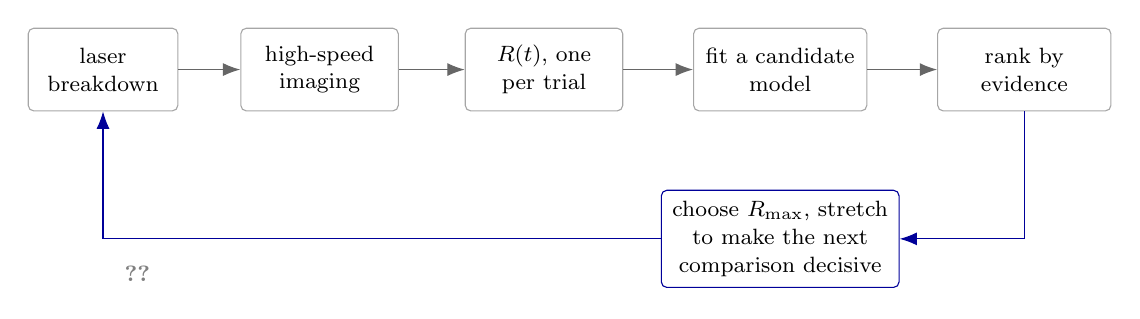
\begin{tikzpicture}[
  box/.style={draw=gray!70,rounded corners=2pt,align=center,inner sep=4pt,minimum height=1.05cm},
  ar/.style={-{Latex[length=2.2mm]},gray!80!black}]
  \node[box,minimum width=1.9cm] (laser) at (0,0) {\footnotesize laser\\[-2pt]\footnotesize breakdown};
  \node[box,minimum width=2.0cm] (image) at (2.75,0) {\footnotesize high-speed\\[-2pt]\footnotesize imaging};
  \node[box,minimum width=2.0cm] (trace) at (5.6,0) {\footnotesize $R(t)$, one\\[-2pt]\footnotesize per trial};
  \node[box,minimum width=2.2cm] (fit) at (8.6,0) {\footnotesize fit a candidate\\[-2pt]\footnotesize model};
  \node[box,minimum width=2.2cm] (rank) at (11.7,0) {\footnotesize rank by\\[-2pt]\footnotesize evidence};
  \foreach \a/\b in {laser/image, image/trace, trace/fit, fit/rank} { \draw[ar] (\a) -- (\b); }
  \node[box,minimum width=2.6cm,draw=blue!60!black] (design) at (8.6,-2.15)
    {\footnotesize choose $R_{\max}$, stretch\\[-2pt]\footnotesize to make the next\\[-2pt]\footnotesize comparison decisive};
  \draw[ar,blue!60!black] (rank.south) |- (design.east);
  \draw[ar,blue!60!black] (design.west) -| (laser.south);
  \node[gray,anchor=west] at (0.15,-2.6) {\footnotesize \cref{sec:design}};
\end{tikzpicture}
\caption{Where this work sits in the measurement chain. A laser nucleates a bubble, imaging
records how its radius changes, and a material model is fitted to that curve. The fitted
stiffness and viscosity are then quoted as material properties. This paper concerns the two
right-hand boxes: which model to believe, and which experiment to run so that the question can
be answered. Ranking on goodness of fit alone does not work here, because a model with more
parameters always fits at least as well as the simpler model inside it.}
\label{fig:pipeline}
\end{figure}

\section{Records and noise model}


Each dataset is a set of repeated laser-induced cavitation events at one temperature,
recorded as $R(t)/R_{\max}$. \Cref{fig:records} shows the mean trace and the trial-to-trial
spread. We use that spread as the measurement noise. It is measured rather than assumed, so
$\chi^2/N \approx 1$ means a model reproduces the record to within experimental
repeatability.

\begin{figure}[htbp]
\centering
\includegraphics[width=\textwidth]{fig_records.pdf}
\caption{Measured records. Line is the mean over trials, band is $\pm$ one standard
deviation across trials at each time. The spread is the noise model.}
\label{fig:records}
\end{figure}

Two samples are excluded before fitting. A trial reading above its own maximum radius is a
tracking failure. And the $t=0$ sample, where every trial agrees exactly, is a definition
rather than a measurement: giving it an error bar would invent an uncertainty and let it
constrain the fit.

Each candidate is evaluated on a log-spaced grid over its own parameters, at one resolution
for every model, so grid luck cannot decide the winner. The evidence is a grid quadrature over
that box. It carries three further pieces: the noise scale marginalized under a half-Cauchy
prior, a redundancy factor down-weighting parameters where a model merely reproduces a simpler
model it contains, and a BIC-style complexity penalty.

Trajectories are compressible~\citep{keller1980bubble}. The incompressible approximation
changes the residuals by a factor of two to four and must not be used for these records.

\section{Method}

Four objects carry the analysis. Each is derived here rather than quoted, because the
choices between them are not neutral and two of the errors this study corrected came from
treating them as interchangeable.

\subsection{The likelihood, and what it assumes}

Each record gives a mean radius $y_i$ at time $t_i$ over $18$ trials, with the
trial-to-trial standard deviation $s_i$ as the noise estimate. Modeling the observations
as independent and Gaussian about the prediction $m_i(\theta)$,
%
\begin{equation}
p(y \mid \theta) = \prod_i \frac{1}{\sqrt{2\pi}\,\sigma_i}
  \exp\!\left[-\frac{(y_i - m_i(\theta))^2}{2\sigma_i^2}\right],
\qquad
-2\log p = \chi^2(\theta) + \sum_i \log\!\big(2\pi\sigma_i^2\big).
\label{eq:likelihood}
\end{equation}

Three assumptions are buried here and each is separately checkable. \emph{Gaussianity} is
the weakest claim, and is reasonable because $y_i$ is a mean over $18$ trials.
\emph{Known $\sigma_i$} is not innocuous: using the sample spread as the true deviation
understates uncertainty. \Cref{sec:beta} handles it by giving the noise scale a prior and
integrating it out. \emph{Independence} is the one that fails: the
diagonal covariance in~\eqref{eq:likelihood} says each residual carries fresh information,
and \cref{sec:limitations} measures a lag-one autocorrelation of $0.90$.

The deviations are not constant across the record. Optical tracking degrades where the wall
moves fastest, so the variance is inflated by a logistic weight in the strain rate,
$\sigma_i^2 = s_i^2/w_i$ with
$w = w_0 + (1-w_0)\,\mathrm{logit}^{-1}\!\big(\kappa(\dot\varepsilon_{\rm th} -
|\dot\varepsilon_i|)/\dot\varepsilon_{\rm th}\big)$. This is a statement about the
measurement, not the model, and it is why $\chi^2/N$ is dominated by the late record where
the weights are large.


\begin{figure}[t]
\centering
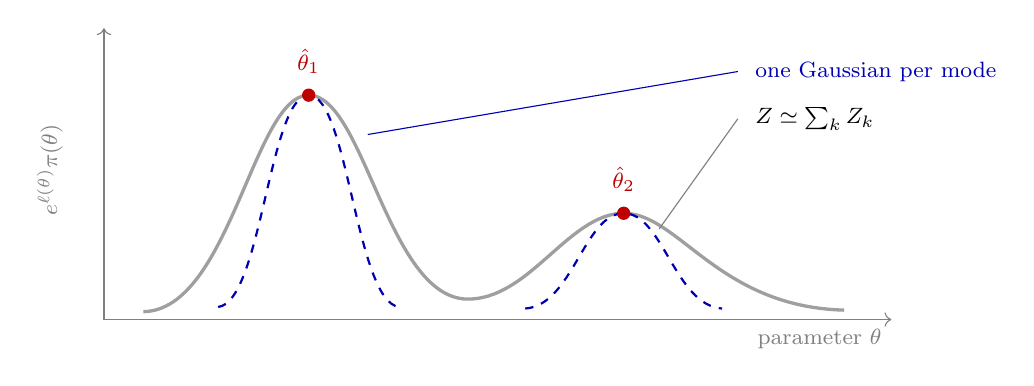
\begin{tikzpicture}[scale=1.0]
  \draw[->,gray] (0,0) -- (10.0,0) node[anchor=north east] {\footnotesize parameter $\theta$};
  \draw[->,gray] (0,0) -- (0,3.7);
  \node[gray,rotate=90,anchor=south] at (-0.4,1.9) {\footnotesize $e^{\ell(\theta)}\pi(\theta)$};
  % the integrand: two humps, drawn as beziers
  \draw[gray!75,very thick]
    (0.5,0.10) .. controls (1.6,0.12) and (1.9,2.85) .. (2.6,2.85)
    .. controls (3.3,2.85) and (3.6,0.30) .. (4.6,0.26)
    .. controls (5.4,0.24) and (5.9,1.35) .. (6.6,1.35)
    .. controls (7.3,1.35) and (7.8,0.16) .. (9.4,0.12);
  % Gaussian fits, drawn only near each mode
  \draw[blue!70!black,thick,dashed]
    (1.45,0.16) .. controls (2.0,0.22) and (2.1,2.85) .. (2.6,2.85)
    .. controls (3.1,2.85) and (3.2,0.22) .. (3.75,0.16);
  \draw[blue!70!black,thick,dashed]
    (5.35,0.14) .. controls (5.95,0.18) and (6.1,1.35) .. (6.6,1.35)
    .. controls (7.1,1.35) and (7.25,0.18) .. (7.85,0.14);
  \fill[red!75!black] (2.6,2.85) circle (2.4pt);
  \fill[red!75!black] (6.6,1.35) circle (2.4pt);
  \node[red!75!black,anchor=south] at (2.6,3.0) {\footnotesize $\hat\theta_1$};
  \node[red!75!black,anchor=south] at (6.6,1.5) {\footnotesize $\hat\theta_2$};
  \node[blue!70!black,anchor=west] at (8.15,3.15) {\footnotesize one Gaussian per mode};
  \node[anchor=west] at (8.15,2.55) {\footnotesize $Z\simeq\sum_k Z_k$};
  \draw[blue!70!black,thin] (8.05,3.15) -- (3.35,2.35);
  \draw[gray,thin] (8.05,2.55) -- (7.05,1.15);
\end{tikzpicture}
\caption{The Laplace expansion, and why the evidence is summed over modes. The integrand
$e^{\ell}\pi$ is expanded about each maximum as a Gaussian, whose height and width give that
mode's contribution $Z_k$ in closed form; the evidence is $\sum_k Z_k$, computed as a
\texttt{logsumexp} over the distinct endpoints a multistart finds. Taking only the best mode
discards the rest of the integral, which is the difference between an integral criterion and a
minimum: a missed mode biases the total slightly, where a missed basin corrupts a minimum
entirely. This is why \texttt{fit\_candidate} returns every distinct endpoint rather than its
winner.}
\label{fig:laplace}
\end{figure}

\subsection{Integrating out the noise scale}
\label{sec:beta}

Rather than trust $s_i$, introduce a single scale $\beta$ multiplying every deviation,
$\sigma_i \to \beta\sigma_i$. Substituting into~\eqref{eq:likelihood},
%
\begin{equation}
\log p(y \mid \theta, \beta)
= -\frac{\chi^2(\theta)}{2\beta^2} - N\log\beta + \text{const},
\label{eq:beta}
\end{equation}
%
which depends on the data only through $\chi^2$ and $N$. That is what makes the
marginalization cheap: the forward model never re-enters, so
%
\begin{equation}
\log p(y\mid\theta) = \log \int_0^\infty p(y \mid \theta,\beta)\,\pi(\beta)\,\mathrm{d}\beta
\label{eq:marginal-beta}
\end{equation}
%
costs one pass over a quadrature grid rather than one solve per node. With the half-Cauchy
prior $\pi(\beta) = (2/\pi)/(1+\beta^2)$ the integral is done numerically on
$\beta\in[0.05,10]$.

Why marginalize rather than fit $\beta$? Profiling at its best value gives
$-\tfrac12 N\,[1 + \log(\chi^2/N)]$, and marginalizing is always smaller. The gap is an
Occam penalty: a model that fits only by inflating its own error bars is charged for the
inflation. Fitting $\beta$ would hand that flexibility over for free.


\begin{figure}[t]
\centering
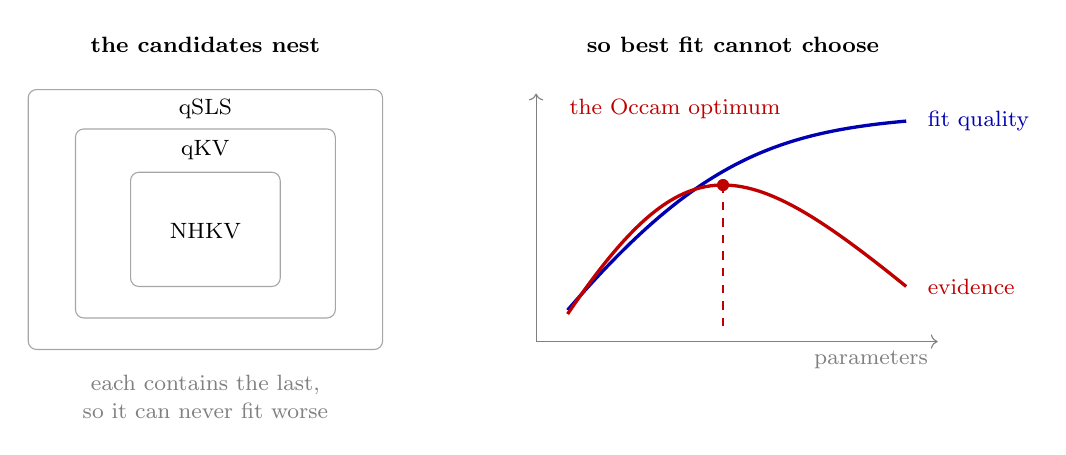
\begin{tikzpicture}[scale=1.0]
\begin{scope}
  \node[anchor=south] at (2.4,3.9) {\footnotesize\textbf{the candidates nest}};
  \draw[rounded corners=3pt,gray!70] (0.15,0.25) rectangle (4.65,3.55);
  \draw[rounded corners=3pt,gray!70] (0.75,0.65) rectangle (4.05,3.05);
  \draw[rounded corners=3pt,gray!70] (1.45,1.05) rectangle (3.35,2.5);
  \node at (2.4,1.75) {\footnotesize NHKV};
  \node at (2.4,2.78) {\footnotesize qKV};
  \node at (2.4,3.3) {\footnotesize qSLS};
  \node[gray,anchor=north,align=center] at (2.4,0.05)
    {\footnotesize each contains the last,\\[-2pt]\footnotesize so it can never fit worse};
\end{scope}
\begin{scope}[xshift=6.6cm]
  \node[anchor=south] at (2.5,3.9) {\footnotesize\textbf{so best fit cannot choose}};
  \draw[->,gray] (0,0.35) -- (5.1,0.35) node[anchor=north east] {\footnotesize parameters};
  \draw[->,gray] (0,0.35) -- (0,3.5);
  \draw[blue!70!black,very thick] (0.4,0.75) .. controls (2.0,2.6) and (3.0,3.0) .. (4.7,3.15);
  \draw[red!75!black,very thick] (0.4,0.7) .. controls (1.9,2.9) and (2.6,2.75) .. (4.7,1.05);
  % on the curve's actual maximum, computed from its control points rather than eyeballed:
  % the marker was sitting above the curve, which is the one thing this panel must get right
  \fill[red!75!black] (2.374,2.338) circle (2.2pt);
  \draw[red!75!black,thin,dashed] (2.374,2.338) -- (2.374,0.45);
  % beyond the end of each curve, so nothing can run into the label above the maximum
  \node[blue!70!black,anchor=west] at (4.85,3.15) {\footnotesize fit quality};
  \node[red!75!black,anchor=west] at (4.85,1.05) {\footnotesize evidence};
  % above the maximum, where neither curve reaches. Two earlier placements failed: beneath
  % the axis it collided with the axis label, and to the left it lay across the evidence
  % curve itself. The dashed drop-line is what ties it to the point.
  \node[red!75!black,anchor=west] at (0.3,3.3) {\footnotesize the Occam optimum};
\end{scope}
\end{tikzpicture}
\caption{Why this study ranks by evidence and not by fit. The constitutive candidates nest --
\texttt{NHKV} is \texttt{qKV} at zero stiffening and \texttt{qSLS} at zero relaxation time --
so a larger model can never fit worse, and the best-fitting candidate is simply the most
flexible one. The evidence adds the Occam factor of \cref{fig:occam}, which charges a
model for prior volume the data does not use, and so turns a monotone quantity into one with
an interior maximum. Everything downstream depends on that penalty being computed correctly,
which is why the pathology in \cref{fig:occam} matters.}
\label{fig:fitvsevidence}
\end{figure}

\subsection{Why the evidence, and not the best fit}

From Bayes' theorem, the posterior odds between two models are the prior odds times the
ratio of
%
\begin{equation}
Z_M = p(y \mid M) = \int p(y \mid \theta, M)\,\pi(\theta \mid M)\,\mathrm{d}\theta .
\label{eq:evidence}
\end{equation}
%
This is the only quantity that answers ``which model should I believe'' without an arbitrary
complexity penalty. Comparing best fits cannot: a nested model never fits worse than the model
containing it, so $\chi^2$ ranks by flexibility.

Information criteria add a penalty -- $2k$ for AIC, $k\log N$ for BIC. But BIC is an
asymptotic approximation to $-2\log Z$ assuming a regular, well-identified model with $N$
large, and \cref{sec:identifiability} shows this one is not identified in a direction. The
integral itself assumes none of that.

The penalty appears explicitly on expanding~\eqref{eq:evidence} about the maximum. With
$\hat\theta$ the best fit, $H = -\nabla^2\log p(y\mid\theta)$ evaluated there, and
$\theta = \hat\theta + \delta$,
%
\begin{equation}
Z_M \simeq p(y\mid\hat\theta)\,\pi(\hat\theta)\int
  \exp\!\left[-\tfrac12\delta^{\mathsf T}H\delta\right]\mathrm{d}\delta
= \underbrace{p(y\mid\hat\theta)}_{\text{best fit}}\;
  \underbrace{\pi(\hat\theta)\,(2\pi)^{p/2}\,|H|^{-1/2}}_{\text{Occam factor}} .
\label{eq:laplace}
\end{equation}
%
The Gaussian integral is exact for a quadratic $-\log p$, so~\eqref{eq:laplace} is the
Laplace approximation and its error is governed by the third derivative. Reading the second
factor as $\pi(\hat\theta)\times(\text{posterior volume})$ makes its meaning plain: it is
the fraction of the prior the posterior actually occupies, so a model needing fine tuning
pays. This is the sense in which a good fit and a credible model differ, and it is what
Freund and Ewoldt~\citep{freund2015quantitative} argue should replace goodness-of-fit ranking in rheology.

One consequence matters later and is easy to miss. Because $|H|^{-1/2}$ grows as the
posterior broadens, a sloppy direction \emph{raises} the evidence. Model comparison
therefore cannot detect non-identifiability -- it rewards it -- and the two questions must
be asked separately.

\subsection{The prior this study uses}
\label{sec:prior}

Equation~\eqref{eq:evidence} needs $\pi(\theta\mid M)$, and a uniform box would make the
answer depend on where the box was drawn. Two factors are used instead, both computed on
the same grid the quadrature runs over.

The \emph{bottleneck} maps each parameter to $u_j\in[0,1]$ in logarithms, then takes the
harmonic mean $H(\theta) = p\big/\sum_j u_j^{-1}$. Logarithms because the parameters span
decades, where a linear map would encode the bounds rather than the physics.

The harmonic mean beats the arithmetic one here precisely because it is dominated by its
smallest argument. A parameter driven to the bottom of its range drags the whole prior down.
The reasoning: a parameter the data pushed to a boundary is one the model did not need.

The \emph{redundancy} weight asks whether a model merely emulates a simpler one it contains.
For a candidate and each nested child, the relative stress mismatch $F$ is mapped by
$F^n/(F^n + \tau^n)$ against the resolvable scale $\tau$. That gives a number near $0$ when
the parent imitates the child, approaching $1$ when it does something genuinely different.

The weight is the \emph{minimum} over children. A model that can imitate any one simpler
model is redundant there, however different it looks from the rest.

\subsection{The Fisher information, and what its eigenvectors are}
\label{sec:identifiability}

Differentiate $-\log p$ twice at fixed data and take the expectation over noise. The term
containing $\partial^2 m$ vanishes because $\mathbb{E}[y_i - m_i] = 0$, leaving
%
\begin{equation}
F_{jk} = \sum_i \frac{1}{\sigma_i^2}
  \frac{\partial m_i}{\partial\theta_j}\frac{\partial m_i}{\partial\theta_k}
= \big(J^{\mathsf T}J\big)_{jk},
\qquad
J_{ij} = \frac{1}{\sigma_i}\frac{\partial m_i}{\partial\theta_j},
\label{eq:fisher}
\end{equation}
%
so the Fisher information is exactly the Gram matrix of the whitened sensitivities -- no
approximation, given~\eqref{eq:likelihood}. Near the optimum
$\Delta\chi^2 \simeq \Delta\theta^{\mathsf T}F\Delta\theta$, so the surface of constant
misfit is the ellipsoid $\Delta\theta^{\mathsf T}F\Delta\theta = c$. Diagonalizing
$F = V\Lambda V^{\mathsf T}$, its axes are the eigenvectors and their half-lengths are
$\sqrt{c/\lambda_k}$: a small eigenvalue is a long axis, a direction along which the data
barely object.

The Cram\'er--Rao bound gives this statistical force. For any unbiased estimator,
$\operatorname{Cov}(\hat\theta) \succeq F^{-1}$, so $F^{-1}$ is the best achievable
covariance and its eigen-decomposition is the confidence ellipsoid. The standard deviation
along direction $k$ is $\lambda_k^{-1/2}$, and the ratio
$\kappa = \lambda_{\max}/\lambda_{\min}$ measures how far the problem is from determining
all directions equally.

Two conventions are load-bearing. Taking $\theta = \log(\text{parameters})$ makes an
eigenvector a power law: moving along $v$ sends $\Delta\log g = v_g t$ and
$\Delta\log\alpha = v_\alpha t$, so $g \propto \alpha^{v_g/v_\alpha}$ and the exponent is
read directly off the components. Second, sensitivities taken with respect to a scaled
coordinate $u_j = (\log\theta_j - a_j)/w_j$ give $\Delta\log\theta_j = w_j\tilde v_j$, so the
exponent is $(w_g\tilde v_g)/(w_\alpha\tilde v_\alpha)$. With box widths of three and four
decades that is a $25\%$ correction. Getting it wrong produced a spurious agreement earlier
in this work.

Finally, $F$ is the observability Gramian of the system augmented with $\dot\theta = 0$:
identifiability and observability are the same statement. The distinction that matters is
\emph{structural} unidentifiability, where $F$ is singular and no data can help, against
\emph{practical} sloppiness, where $F$ is invertible but ill-conditioned. Here
$\lambda_{\min} = 5.2\times10^{-2} \neq 0$ and the profile likelihood has a genuine minimum,
so the problem is the second -- which is why a different experiment can fix it.


\begin{figure}[t]
\centering
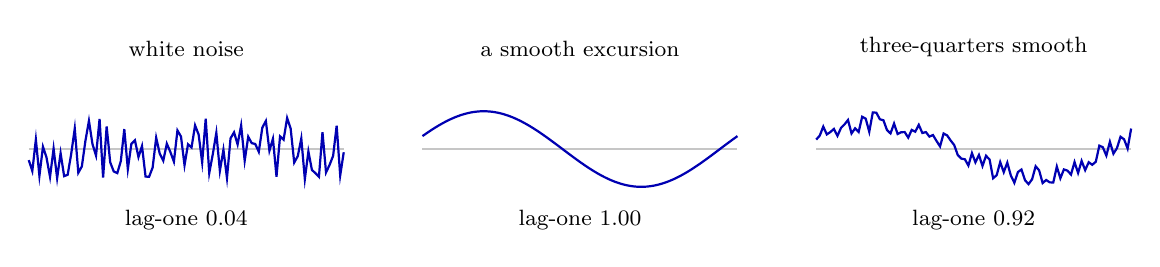
\begin{tikzpicture}[scale=1.0]
\begin{scope}
  \node[anchor=south] at (2.0,1.95) {\footnotesize white noise};
  \draw[gray!45] (0,0.9) -- (4.0,0.9);
  \draw[blue!70!black,thick] plot coordinates {(0.000,0.759) (0.045,0.621) (0.090,1.021) (0.135,0.558) (0.180,0.929) (0.225,0.793) (0.270,0.546) (0.315,0.906) (0.360,0.530) (0.404,0.847) (0.449,0.556) (0.494,0.573) (0.539,0.840) (0.584,1.161) (0.629,0.599) (0.674,0.679) (0.719,1.002) (0.764,1.258) (0.809,0.962) (0.854,0.817) (0.899,1.281) (0.944,0.537) (0.989,1.187) (1.034,0.732) (1.079,0.615) (1.124,0.594) (1.169,0.747) (1.213,1.153) (1.258,0.645) (1.303,0.965) (1.348,1.011) (1.393,0.798) (1.438,0.938) (1.483,0.550) (1.528,0.548) (1.573,0.665) (1.618,1.044) (1.663,0.842) (1.708,0.751) (1.753,0.968) (1.798,0.863) (1.843,0.740) (1.888,1.136) (1.933,1.059) (1.978,0.695) (2.022,0.960) (2.067,0.920) (2.112,1.200) (2.157,1.084) (2.202,0.730) (2.247,1.284) (2.292,0.594) (2.337,0.834) (2.382,1.106) (2.427,0.622) (2.472,0.891) (2.517,0.531) (2.562,1.035) (2.607,1.112) (2.652,0.958) (2.697,1.200) (2.742,0.751) (2.787,1.056) (2.831,0.975) (2.876,0.964) (2.921,0.865) (2.966,1.172) (3.011,1.256) (3.056,0.879) (3.101,1.031) (3.146,0.549) (3.191,1.061) (3.236,1.018) (3.281,1.294) (3.326,1.158) (3.371,0.728) (3.416,0.809) (3.461,1.035) (3.506,0.518) (3.551,0.869) (3.596,0.634) (3.640,0.594) (3.685,0.547) (3.730,1.115) (3.775,0.603) (3.820,0.698) (3.865,0.813) (3.910,1.197) (3.955,0.564) (4.000,0.859)};
  \node[anchor=north] at (2.0,0.25) {\footnotesize lag-one $0.04$};
\end{scope}
\begin{scope}[xshift=5.0cm]
  \node[anchor=south] at (2.0,1.95) {\footnotesize a smooth excursion};
  \draw[gray!45] (0,0.9) -- (4.0,0.9);
  \draw[blue!70!black,thick,smooth,samples=60,domain=0:4]
    plot (\x, {0.9 + 0.48*sin(90*\x + 20)});
  \node[anchor=north] at (2.0,0.25) {\footnotesize lag-one $1.00$};
\end{scope}
\begin{scope}[xshift=10.0cm]
  \node[anchor=south] at (2.0,1.95) {\footnotesize three-quarters smooth};
  \draw[gray!45] (0,0.9) -- (4.0,0.9);
  \draw[blue!70!black,thick] plot coordinates {(0.000,1.020) (0.045,1.070) (0.090,1.185) (0.135,1.086) (0.180,1.116) (0.225,1.155) (0.270,1.067) (0.315,1.168) (0.360,1.213) (0.404,1.269) (0.449,1.098) (0.494,1.163) (0.539,1.116) (0.584,1.310) (0.629,1.285) (0.674,1.119) (0.719,1.365) (0.764,1.361) (0.809,1.278) (0.854,1.265) (0.899,1.141) (0.944,1.098) (0.989,1.223) (1.034,1.091) (1.079,1.114) (1.124,1.115) (1.169,1.045) (1.213,1.143) (1.258,1.120) (1.303,1.207) (1.348,1.104) (1.393,1.115) (1.438,1.058) (1.483,1.078) (1.528,1.003) (1.573,0.933) (1.618,1.097) (1.663,1.073) (1.708,1.008) (1.753,0.950) (1.798,0.824) (1.843,0.778) (1.888,0.770) (1.933,0.690) (1.978,0.848) (2.022,0.731) (2.067,0.825) (2.112,0.685) (2.157,0.814) (2.202,0.767) (2.247,0.529) (2.292,0.567) (2.337,0.734) (2.382,0.606) (2.427,0.727) (2.472,0.564) (2.517,0.471) (2.562,0.608) (2.607,0.640) (2.652,0.504) (2.697,0.454) (2.742,0.516) (2.787,0.681) (2.831,0.630) (2.876,0.468) (2.921,0.507) (2.966,0.477) (3.011,0.475) (3.056,0.677) (3.101,0.528) (3.146,0.641) (3.191,0.626) (3.236,0.576) (3.281,0.734) (3.326,0.596) (3.371,0.749) (3.416,0.632) (3.461,0.732) (3.506,0.700) (3.551,0.738) (3.596,0.943) (3.640,0.923) (3.685,0.817) (3.730,0.992) (3.775,0.841) (3.820,0.912) (3.865,1.056) (3.910,1.024) (3.955,0.906) (4.000,1.160)};
  \node[anchor=north] at (2.0,0.25) {\footnotesize lag-one $0.92$};
\end{scope}
\end{tikzpicture}
\caption{What lag-one autocorrelation measures, and what it does not. Sampled at the $N=201$
points of these records, lag-one is close to a measure of how much of a residual is
\emph{smooth}: white noise gives $0.04$, a single smooth excursion $1.00$, a mixture that is
three-quarters smooth $0.92$. It does not say what made the residual smooth -- model
discrepancy, variation between bubbles and a slow calibration drift are alike in this
statistic. The \texttt{qSLS} residual gives $0.918$; the trial deviations from the mean, with
no model fitted at all, give $0.859$. Most of the smoothness the fit residual shows is
therefore already in the data.}
\label{fig:lagone}
\end{figure}

\subsection{What correlated residuals cost}

Equation~\eqref{eq:likelihood} counts $N$ independent pieces of information. If instead the
residuals have autocorrelation $\rho_k$ at lag $k$, then for a sum of $N$ correlated terms
$\operatorname{Var}(\sum r_i) = N\sigma^2\big(1 + 2\sum_k (1-k/N)\rho_k\big)$, so the
information is that of
%
\begin{equation}
N_{\rm eff} = \frac{N}{1 + 2\sum_{k\ge1}\rho_k}
\label{eq:ess}
\end{equation}
%
independent samples, and parameter uncertainties are understated by
$\sqrt{N/N_{\rm eff}}$. The sum is truncated at the first negative $\rho_k$ -- Geyer's
initial positive sequence -- because the long tail is estimated from few pairs each and
contributes sampling error rather than signal.

The correct remedy is a covariance with off-diagonal terms, not a larger $\sigma$. Taking
$C_{ij} = \sigma_i\sigma_j\exp(-|t_i-t_j|/\tau)$, the Cholesky factor $C = LL^{\mathsf T}$
gives the generalized least squares form
%
\begin{equation}
-2\log p = r^{\mathsf T}C^{-1}r + \log|C| + \text{const}
= \|L^{-1}r\|^2 + 2\sum_k \log L_{kk} + \text{const},
\end{equation}
%
which is what \texttt{FieldObservation} computes. Inflating $\sigma$ instead would treat
structure as noise: it widens the error bars while leaving the parameter estimates biased,
which is the failure Brynjarsd\'ottir and O'Hagan warn about.

\subsection{Which design criterion, and why they disagree}
\label{sec:criteria}

An experiment is chosen by a scalar summary of $F$. The classical family is
%
\begin{equation}
\text{D: } \max \det F, \qquad
\text{A: } \min \operatorname{tr} F^{-1}, \qquad
\text{E: } \max \lambda_{\min}, \qquad
\text{c: } \min\, c^{\mathsf T}F^{-1}c .
\end{equation}
%
D minimizes the volume of the confidence ellipsoid, A its mean squared axis length, E its
longest axis, and c the variance of one nominated combination. They rank designs differently
because they summarize the same spectrum differently. The choice states what one wants to
learn.

For identifiability the relevant fact is a scaling argument. A design change that only
amplifies signal -- more samples, less noise, a larger bubble -- sends $F \to sF$. Then
$\det F \to s^p\det F$ and $\lambda_{\min}\to s\lambda_{\min}$, so D and E both improve,
while
%
\begin{equation}
\kappa = \frac{\lambda_{\max}}{\lambda_{\min}} \quad\text{is unchanged.}
\end{equation}
%
Degeneracy is a property of the eigen\emph{vectors}, not the eigenvalues. Only a design that
rotates them can remove it. That is why the E-optimal search preferred a larger bubble while
conditioning preferred a gentler collapse: more signal against better separation.

The c-optimal choice carries a small trap. Nominating $c$ as the sloppy direction \emph{of the
present design} optimizes for a direction that moves once the design changes. In this study
that criterion recommended the opposite of the right answer.

When the model itself is in doubt, none of these apply: all presuppose the model whose $F$ is
being computed. T-optimality asks instead for the design maximizing the discrepancy
between rival predictions, $\max_\xi \|m_1(\hat\theta_1;\xi) - m_2(\hat\theta_2;\xi)\|$, and
privileges neither.

\section{Identifiability of the constitutive parameters}

The winner fits, but not every parameter it contains is measured by these data.

\subsection*{Why the trade exists}

Write $\hat g = G/p_\infty = 1/\mathrm{Ca}$ for the nondimensional modulus and
$\lambda = R_{\mathrm{eq}}/R$ for the stretch the stress law sees. The equilibrium stress
the Maxwell arm relaxes toward is
%
\begin{equation}
Z_e = R^3\left[\tfrac{3\alpha-1}{2}\,\hat g\,P(\lambda) + 2\alpha\,\hat g\,Q(\lambda)\right],
\qquad
\begin{aligned}
P(\lambda) &= 5 - \lambda^4 - 4\lambda,\\
Q(\lambda) &= \tfrac{27}{40} + \tfrac{1}{8}\lambda^8 + \tfrac{1}{5}\lambda^5 + \lambda^2 - \tfrac{2}{\lambda}.
\end{aligned}
\label{eq:Ze}
\end{equation}
%
Collecting powers of $\alpha$ separates it into two terms with different parameter
dependence,
%
\begin{equation}
Z_e = \hat g\,\alpha\,A(\lambda) + \hat g\,B(\lambda),
\qquad
A = R^3\!\left[\tfrac32 P + 2Q\right],
\qquad
B = -\tfrac12 R^3 P .
\label{eq:split}
\end{equation}
%
This is exact; it reproduces the implemented expression to $2.5\times10^{-14}$ over random
states. Only the first term carries $\alpha$, so $\hat g\alpha$ and $\hat g$ are separately
determined only while \emph{both} terms contribute.

They do not, at depth. As $\lambda$ grows, $Q \to \tfrac18\lambda^8$ dominates every other
term in either bracket, so $A \to \tfrac14 R^3\lambda^8$ while $B \sim \tfrac12 R^3\lambda^4$,
and
%
\begin{equation}
Z_e \;\longrightarrow\; \tfrac14\,\hat g\,\alpha\,R^3\lambda^8 ,
\end{equation}
%
a function of the \emph{product} $\hat g\alpha$ alone. The likelihood cannot then distinguish
a soft material that stiffens sharply from a stiff one that barely stiffens. Holding $Z_e$
fixed in~\eqref{eq:split} gives the trade in closed form,
%
\begin{equation}
\frac{\partial \log \hat g}{\partial \log \alpha}
= -\frac{\alpha A}{\alpha A + B}
\;\longrightarrow\; -1 \quad (\lambda \to \infty),
\label{eq:exponent}
\end{equation}
%
and the share of the signal that separates the two parameters is
%
\begin{equation}
\frac{|\hat g B|}{|\hat g \alpha A|} = \frac{|B|}{\alpha|A|} \simeq \frac{2}{\alpha\lambda^4}.
\label{eq:separability}
\end{equation}

Equations~\eqref{eq:exponent} and~\eqref{eq:separability} are what the measurements see.
These records collapse to $\lambda = 2.215$, where~\eqref{eq:exponent} gives $-0.981$ against
$-0.99$ from the Fisher curvature -- a prediction from the constitutive law, not a fit. The
profile likelihood returns $-0.80$ because it averages over a range of $\lambda$, and the
exponent is $-0.861$ at $\lambda = 1.5$. Separability falls as $\lambda^{-4}$: it is $2\%$ of
the signal at $\lambda = 2.2$ and $16\%$ at $\lambda = 1.5$.

\begin{figure}[htbp]
\centering
\includegraphics[width=0.98\textwidth]{fig_separability.pdf}
\caption{The two terms of~\eqref{eq:split} against collapse depth. Left: $\alpha A$, which
depends on the product $g\alpha$, outruns $B$, which carries $g$ alone. Right: their ratio,
the share of the signal that can separate the two parameters, following
$2/(\alpha\lambda^4)$ once the collapse is deep. It is $2\%$ at the depth these records
reach and $16\%$ at $\lambda = 1.5$.}
\label{fig:separability}
\end{figure}

\subsection*{What the Fisher information measures}

For Gaussian observations with known deviations the log-likelihood is
$-\tfrac12\sum_i (y_i - m_i(\theta))^2/\sigma_i^2$ up to a constant, so with the whitened
sensitivity $J_{ij} = \sigma_i^{-1}\partial m_i/\partial\theta_j$ the Fisher information is
exactly $F = J^{\mathsf T}J$, and $\Delta\chi^2 \simeq \Delta\theta^{\mathsf T} F \Delta\theta$.
Taking $\theta$ to be the logarithms of the parameters makes the eigenvectors read as
power-law combinations: along an eigenvector $v$ the ratio $v_g/v_\alpha$ is the exponent
in $g \propto \alpha^{v_g/v_\alpha}$. This is also the observability Gramian of the system
augmented with $\dot\theta = 0$, which is why identifiability and observability are the same
statement here.

One caution, since it caught us. Sensitivities taken with respect to a unit cube
$u_j = (\log\theta_j - a_j)/w_j$, rather than $\log\theta_j$ directly, give eigenvector
components that carry the box widths. Then $\Delta\log\theta_j = w_j\,\tilde v_j$, so the
exponent is $(w_g \tilde v_g)/(w_\alpha \tilde v_\alpha)$, not $\tilde v_g/\tilde v_\alpha$.
With $w$ of three and four decades the two differ by $25\%$.

\begin{figure}[htbp]
\centering
\includegraphics[width=0.98\textwidth]{fig_eigenvectors.pdf}
\caption{What an eigenvector means, shown rather than defined. The parameters are moved the
same distance in $\log$-space along each eigenvector. Along the sloppy direction a $27\%$
change in the modulus, compensated by $38\%$ in the stiffening, leaves the trajectory inside
the measurement noise; along the stiff direction a change of the same size is obvious. The
data cannot see the first and cannot miss the second.}
\label{fig:eigenvectors}
\end{figure}

\begin{figure}[htbp]
\centering
\includegraphics[width=0.98\textwidth]{fig_ellipse.pdf}
\caption{Left: the $95\%$ region from the inverse Fisher information, $10.7$ long and
$0.015$ wide in $\log$-parameters -- an axis ratio of $706$, which is why it draws as a
line, and the analytic slope of $-0.981$ lies along it. Right: the misfit measured by
re-solving at perturbed parameters, not the quadratic approximation. Moving along the stiff
direction costs $10^4$ in $\Delta\chi^2$; moving the same distance along the sloppy one stays
below the $95\%$ threshold, so the parameters may shift by a factor of $e \approx 2.7$
without the data objecting.}
\label{fig:ellipse}
\end{figure}

\paragraph{Modulus and stiffening trade against each other.}
Two independent analyses agree. The Fisher information at the fitted optimum has an
eigenvalue spectrum spanning six decades. The eigenvector of its smallest eigenvalue is almost
purely a shear-modulus-against-stiffening direction: weights $-0.796$ and $+0.604$, against
contributions of $-0.003$ and $-0.032$ from viscosity and relaxation time.
Separately, profiling the likelihood in $\alpha$ -- fixing it and re-optimizing everything
else -- gives $g \propto \alpha^{-0.80}$ across two decades. Sampling the posterior gives a
third, independent measurement: its widest direction is
$(-0.682,\,+0.002,\,-0.082,\,+0.727)$ in the logarithms of
$(g, \mu, \lambda_1, \alpha)$, and $\log g$ is $98.7\%$ anticorrelated with $\log\alpha$.

The three exponents are $-0.99$ from local curvature, $-0.94$ from the posterior covariance,
and $-0.80$ from the profile. They agree the trade is near-reciprocal and disagree in the
third digit. That is expected rather than troubling: the valley is curved, so a curvature
estimate at one point and a chord across two decades measure different slopes. The correlation
is the more robust statement.

So viscosity and relaxation time are cleanly determined, while modulus and stiffening are
constrained only in combination. The identifiable quantity is closer to $g\,\alpha^{0.8}$
than to either alone, and a fitted $\alpha$ should be reported with its correlation to $g$
rather than as an independent material property.

\begin{figure}[htbp]
\centering
\includegraphics[width=0.62\textwidth]{fig_valley.pdf}
\caption{$\chi^2/N$ over the modulus--stiffening plane, at the fitted viscosity and
relaxation time. The dashed line is $g \propto \alpha^{-0.80}$, predicted from the Fisher
curvature at a single point; it lies along the floor of the valley. Four ``best fits'' from
four methods are strung out along that floor rather than disagreeing with one another. The
white region at upper right is where the model is not physical.}
\label{fig:valley}
\end{figure}

\Cref{fig:valley} shows why the four estimates in this study disagree about $g$ by an order of
magnitude while agreeing about the fit. They are different points on the floor of one
flat-bottomed trench.

\paragraph{The stiffening is nonetheless identified, once the prior allows it.}
Sampling with the ceiling on $\alpha$ placed at $1$, $10$ and $100$:

\begin{center}
\begin{tabular}{cccc}
\toprule
ceiling & log evidence & median $\alpha$ & $97.5\%$ \\
\midrule
$1$ & $2162.9$ & $0.85$ & $0.97$ \\
$10$ & $2173.9$ & $6.37$ & $9.04$ \\
$100$ & $2172.4$ & $5.27$ & $8.73$ \\
\bottomrule
\end{tabular}
\end{center}

Widening the prior tenfold moves the median only from $6.37$ to $5.27$, and the evidence by
$1.5$ out of $2173$. So $\alpha$ is identified near $5$, with $97.5\%$ of posterior mass below
about $9$. A prior-dominated parameter would have tracked its bound. The ceiling of
$1$ shows what genuine truncation looks like: the median pins against it and $11$ log units
of evidence are lost.

This corrects a natural reading of the profile likelihood alone, which appears flat to the
boundary only because the boundary sits where the posterior's upper tail does.

\begin{figure}[htbp]
\centering
\includegraphics[width=0.98\textwidth]{fig_identifiability.pdf}
\caption{Left: the Fisher spectrum at the optimum, six decades between the stiffest and
sloppiest directions, with the sloppiest being modulus against stiffening. Right: the
posterior for $\alpha$ against the ceiling imposed on its prior. It tracks the ceiling while
truncated and departs from it once the ceiling is loose, which is what distinguishes an
identified parameter from a prior-driven one.}
\label{fig:identifiability}
\end{figure}

\section{Results}

\cref{tab:fits} and \Cref{fig:fits} give the outcome. The quadratic Zener model
\texttt{qSLS} -- strain-stiffening elasticity with stress relaxation -- wins at every
temperature. The ordering beneath it separates into three tiers: models with both
ingredients, models with relaxation only, and memoryless models.

\begin{table}[htbp]
\centering
\caption{Best $\chi^2/N$ \emph{on the selection grid} by model class -- the best node, not the best fit; \cref{sec:fitquality} refits and reaches $0.962$ for qSLS at \SI{15}{\celsius}. Values near $1$ indicate a fit within
experimental repeatability.}
\label{tab:fits}
\begin{tabular}{lccc}
\toprule
& \SI{15}{\celsius} & \SI{23}{\celsius} & \SI{33}{\celsius} \\
\midrule
\texttt{qSLS} (stiffening $+$ relaxation) & \textbf{1.35} & \textbf{1.33} & \textbf{1.23} \\
\texttt{SLS} (relaxation, linear elasticity) & 2.94 & 1.85 & 1.41 \\
viscoelastic fluids & 5.3--5.7 & 4.5--4.7 & 1.9--2.1 \\
memoryless & 12.6--16.7 & -- & -- \\
\bottomrule
\end{tabular}
\end{table}

\begin{figure}[htbp]
\centering
\includegraphics[width=\textwidth]{fig_fits.pdf}
\caption{Best $\chi^2/N$ on the selection grid for every candidate, all three temperatures, logarithmic scale.
The dashed line is the measurement-noise floor.}
\label{fig:fits}
\end{figure}

\Cref{fig:winner} overlays the winning model on the data it was selected against.

\begin{figure}[htbp]
\centering
\includegraphics[width=\textwidth]{fig_winner.pdf}
\caption{The selected model against the measured band it was fitted to.}
\label{fig:winner}
\end{figure}

\subsection{Reading the posteriors}

The model posteriors saturate. The winner takes essentially all the mass and the runners-up
are reported as $10^{-29}$ or smaller. Do not read these magnitudes literally.

Evidence differences scale with sample count. With roughly $3600$ samples, a modest
per-sample difference in fit compounds into an astronomical Bayes factor. The defensible
reading is ordinal: the winner is decisive and the ordering means something, the magnitudes
do not. Quote the residual $\chi^2/N$.

\subsection{How good are the fits, really?}
\label{sec:fitquality}

The table above reports the best $\chi^2/N$ found on the evaluation grid. Two questions
follow, with different answers. How well does the winning model fit? And how much does a good
$\chi^2/N$ entitle us to claim?

\paragraph{The grid understates the fit.}
The model-selection grid evaluates each candidate at log-spaced parameter nodes, so its
best value is the best \emph{node}, not the best fit. Refitting each model to the
\SI{15}{\celsius} record by multistart Gauss--Newton with analytic Jacobians -- eight
starts from a Latin hypercube over the wide prior box, taking the lowest -- gives:

\begin{center}
\begin{tabular}{lcccccc}
\toprule
model & parameters & $\chi^2/N$ & lag-one $\rho$ & $N_{\rm eff}$ & $\chi^2/N_{\rm eff}$ & inflation \\
\midrule
qSLS & $4$ & $\mathbf{0.962}$ & $0.918$ & $10.3$ & $18.9$ & $4.43$ \\
SLS  & $3$ & $1.984$ & $0.932$ & $7.1$  & $56.6$ & $5.34$ \\
qKV  & $3$ & $20.18$ & $0.948$ & $13.4$ & $302$  & $3.87$ \\
NHKV & $2$ & $20.16$ & $0.948$ & $13.4$ & $302$  & $3.87$ \\
\bottomrule
\end{tabular}
\end{center}

At its true optimum qSLS reaches $\chi^2/N = 0.96$ rather than the grid's $1.35$, which
confirms in a second way that the tabulated residuals are ceilings. The ordering is
unchanged, and the gaps are large: relaxation without stiffening doubles the residual, and
both memoryless models sit twenty times above it.

\paragraph{Stiffening buys nothing without relaxation.}
qKV and NHKV differ only by the stiffening exponent $\alpha$, and they fit identically:
$20.18$ against $20.16$, one part in a thousand on a residual twenty times too large. The
strain-stiffening term is decisive alongside a relaxation mode and worth nothing without one.

That is sharper than the evidence ranking alone. It is not that qKV is a worse model than
qSLS; its extra parameter does no work at all. It also explains why the temperature trend is
carried by the interaction of the two mechanisms rather than by either alone.

\paragraph{But $\chi^2/N \approx 1$ does not mean the fit is within noise.}
The statistic $\chi^2/N$ compares the residual to its expectation under the assumption that
the $N$ residuals are independent draws of known scale. They are not. The lag-one
autocorrelation of the qSLS residual is $0.918$, and by the Geyer initial-positive-sequence
estimator~\citep{geyer1992practical} of~\eqref{eq:ess} the $201$ samples carry the information of about
$N_{\rm eff} = 10$ independent ones. Dividing by that count instead gives $18.9$.

That number is not a calibrated test. For correlated residuals the correct statistic is
$r^{\mathsf T}\Sigma^{-1}r$ with the true covariance, not $\chi^2$ rescaled by an effective
count. But its message is robust, and it is the opposite of the headline's.

A residual with $\rho = 0.918$ is not noise the model failed to average away. It is
\emph{structure} the model does not contain. The fit is excellent in that no candidate does
better, and not excellent in that it is inconsistent with the measurement error.

\paragraph{The classical test agrees, and says more.} The argument above rests on lag-one
autocorrelation, which \cref{sec:limitations} shows is a blunt instrument. There is a standard
test for the same question and these records already carry what it needs: replicates. The
trial spread at each time is \emph{pure error}, costing no model, so the residual of the mean
splits into that and what the model cannot follow,
%
\begin{equation}
F = \frac{J\sum_i (\bar y_i - \hat y_i)^2 \,/\, (k-p)}
         {(J-1)\sum_i s_i^2 \,/\, k(J-1)} ,
\label{eq:lackoffit}
\end{equation}
%
with $J$ trials at $k$ times and $p=4$ parameters. The records do not carry equal replication:
$J$ is $18$, $14$ and $7$.

\begin{center}
\begin{tabular}{lcccccc}
\toprule
record & $J$ & $\chi^2/N$ & pure error & lack of fit & $F$ & corrected \\
\midrule
\SI{15}{\celsius} & $18$ & $0.973$ & $5.20\times10^{-4}$ & $7.36\times10^{-3}$ & $\mathbf{14.2}$ & $\mathbf{23.3}$ \\
\SI{23}{\celsius} & $14$ & $1.017$ & $1.86\times10^{-3}$ & $5.47\times10^{-3}$ & $2.9$ & $4.8$ \\
\SI{33}{\celsius} & $7$ & $1.130$ & $1.91\times10^{-3}$ & $6.23\times10^{-3}$ & $3.3$ & $5.4$ \\
\bottomrule
\end{tabular}
\end{center}

\noindent Degrees of freedom are $197$ against $3417$ at \SI{15}{\celsius} and fall with $J$
elsewhere, so the five percent critical value is near $1.2$ throughout. Every record shows lack
of fit. The conclusion is the one above, reached with none of the same machinery.

Two things make it worth the page. It gets the factor of $J$ right by construction --- the fit
compares the \emph{mean} of the trials against the spread \emph{between} them, and the $J$ in
the numerator is that missing $\sqrt{J}$ --- and it is conservative in a direction we can
quantify: \SI{39.3}{\percent} of the trial variance is bubble-to-bubble parameter spread rather
than measurement, so pure error is inflated and the corrected column divides that share out.

It also separates the records, which lag-one does not: those values are $0.919$, $0.968$ and
$0.911$, effectively identical. Two things drive the separation and both are real.
\SI{15}{\celsius} repeats itself about three times more tightly, and it was run with more than
twice the replicates of \SI{33}{\celsius} --- replication is what buys power to detect lack of
fit, so the $F$ column correctly rewards it. Removing the replicate factor, the systematic
misfit variance stands at $0.79$, $0.21$ and $0.47$ of pure error, so the ordering survives but
the spread is milder than $14.2$ against $3.3$ suggests.

The strongest evidence that the model is incomplete therefore comes from the record with the
best apparatus and the most repeats, not from the worst fit.

The $p$-value is not usable: $F$ assumes independent errors across time and these are
correlated at $0.918$. The ratio needs no such assumption, and is read here as an effect size.

Three things follow, and they should be read together.

\begin{enumerate}
\item \emph{The ranking survives.} Refitting under a correlated likelihood with a Cholesky
whitening of an estimated AR(1) covariance changes the qSLS--SLS evidence gap by $3\%$. What
the correlation destroys is the absolute claim, not the comparison, and the comparison is
what the study is for.
\item \emph{The denominator is the wrong yardstick.} The scale $\sigma_i$ is the
trial-to-trial spread. Much of that is variation in the parameters between bubbles, not error
in measuring any one of them. A $\chi^2$ formed against it is not comparing the model to
measurement precision at all.
\item \emph{The misfit is in the early record}, not where the tracking is hardest.
Restricting the fit to a later window makes $\chi^2/N$ worse, $0.97$ to $1.95$, and does not
whiten the residual. The structure cannot be excised by discarding the awkward part of the
record.
\end{enumerate}

The honest summary: qSLS is the best available description of these records by a wide
margin, it is measurably incomplete, and the size of what is missing is better read from the
residual's correlation than from its magnitude.

\subsection{What the trial spread actually is}
\label{sec:latent}

The likelihood of \cref{sec:beta} treats the residuals as independent draws whose scale is
the trial-to-trial spread $s_i$. Two assumptions are buried in that, and both are wrong in
ways that matter for how the numbers above should be read.

\paragraph{Part of the spread is the parameters, not the measurement.}
If the $18$ trials differed only by measurement error, their deviations from the trial mean
would be white and point nowhere in particular. They do neither.

The singular spectrum of the $18 \times 201$ deviation matrix puts $53.9\%$ of the variance in
one component, where white noise would give $5.9\%$. Projecting each deviation onto the span
of $G = \partial (R/R_{\max})/\partial\theta$ for the six parameters
$(R_0, R_{\rm eq}, g, \mu, \lambda_1, \alpha)$ captures $39.3\%$ of the variance against a
chance level of $6/201 = 3.0\%$. Noise does not align with a six-dimensional subspace of a
$201$-dimensional space by accident.

The physical reading is that each bubble has its own parameters, drawn from a population:
$\theta_j \sim \mathcal{N}(\theta_{\rm pop}, \Sigma)$. The mean trace then has covariance
%
\begin{equation}
C \;=\; \frac{1}{J}\Big(G\,\Sigma\,G^{\mathsf T} \;+\; \sigma^2_{\rm meas} I\Big),
\label{eq:hierarchical}
\end{equation}
%
low rank plus diagonal rather than diagonal. Note that $\Sigma$ itself is not estimable here.
Regressing the deviations onto $G$ inherits the $g$--$\alpha$ degeneracy of
\cref{sec:identifiability} and returns $\mathrm{sd}(\log g) = 159$. But only the prediction
covariance $G\Sigma G^{\mathsf T}$ enters~\eqref{eq:hierarchical}, and that is the sample
covariance of the projected deviations, which needs no inversion.

\paragraph{It is not what makes the residuals correlated.}
The natural hypothesis is that the lag-one correlation of the fit residual is this same
effect. Whitening by~\eqref{eq:hierarchical} tests it directly:

\begin{center}
\begin{tabular}{lcc}
\toprule
covariance & $\chi^2/N$ & lag-one $\rho$ \\
\midrule
diagonal (independent) & $17.54$ & $0.758$ \\
hierarchical, \eqref{eq:hierarchical} & $21.96$ & $\mathbf{0.516}$ \\
\bottomrule
\end{tabular}
\end{center}

The correlation falls by about a third, and most of it survives. $\chi^2$ gets \emph{worse},
so the residual sits in directions where $C$ is small. The dominant term is model-form error,
not variation between bubbles. Both effects are real and the model-error one is larger, which
separates two things \cref{sec:limitations} had conflated.

\begin{figure}[htbp]
\centering
\includegraphics[width=\textwidth]{fig_trial.pdf}
\caption{What the trial spread is, and what it does not explain. Left: the singular
spectrum of the eighteen trial deviations. Independent measurement error would put an equal
share in every component (dashed); instead the leading one carries $54\%$, and $39\%$ of
the total lies in the six-dimensional span of $\partial R/\partial\theta$ against a $3\%$
chance level. Right: the autocorrelation of the qSLS fit residual before and after whitening
by the hierarchical covariance~\eqref{eq:hierarchical}, with the white-noise band shaded. If
the correlation were caused by variation between bubbles, whitening would flatten it into
that band. It removes about a third and leaves the rest, so the remainder is structure the
model does not contain.}
\label{fig:trial}
\end{figure}

\paragraph{Which precision $\chi^2/N$ is measured against.}
The same computation exposes a factor of $J = 18$ in the meaning of the headline number. The
data is the \emph{mean} of $18$ trials, but $s_i$ is the spread \emph{between} trials, and the
standard error of the mean is smaller by $\sqrt{18} = 4.24$. From the identical residual,
%
\begin{equation*}
\chi^2/N = 0.974 \;\;\text{against the trial spread},
\qquad
\chi^2/N = 17.54 \;\;\text{against the standard error of the mean}.
\end{equation*}
%
Both are meaningful, and they answer different questions. \emph{The model reproduces the
record to within the scatter between individual experiments} is true, and is the claim this
document makes. \emph{The model is statistically adequate} is false: against the precision the
$18$-trial mean actually carries, it is off by a factor of seventeen. The noise-scale
marginalization of \cref{sec:beta} absorbs the difference -- the implied $\beta \approx 0.24$
lies inside its prior -- so the evidence ranking is undisturbed. What changes is what a
residual near one entitles one to say.

\paragraph{What lag-one does and does not measure.} The inference above -- that whitening
removes a third of the correlation and the remainder is structure the model lacks -- rules
out variation between bubbles, and nothing more. Lag-one autocorrelation at $N = 201$
samples is close to a measure of how much of a residual is \emph{smooth}, not of what made
it smooth: sampled at this density, white noise gives $0.04$, a single sine period gives
$1.00$, a smooth random curve gives $0.999$, and a mixture that is $80\%$ smooth gives
$0.944$. A value of $0.918$ says the residual is roughly three-quarters smooth structure. It
does not say whose.

That matters because the trial deviations from the mean -- pure measurement variation, with
no model fitted at all -- carry lag-one $0.859$ (median over the eighteen trials, range
$0.725$ to $0.890$). Most of the smoothness the fit residual shows is already present in the
data before any model is involved. Whitening by the hierarchical covariance removes the part
of it that lies along $\partial R/\partial\theta$, which is why it removes only a third; the
rest is smooth in the data for reasons the parameter sensitivities cannot represent, and
model-form error is one candidate among several rather than the established remainder.

The searches of \cref{sec:enrich} were run on the stronger reading, and their negative
results are consistent with the weaker one.

\subsection{What to enrich, and how it would have to be judged}
\label{sec:enrich}

The previous section leaves a specific defect: the residual carries structure the model does
not contain, and it is not accounted for by variation between bubbles. The natural suspect is
the assumption of a \emph{single} relaxation time, which is strong for a crosslinked
biopolymer whose relaxation is in reality distributed. Two enrichments follow from that
suspicion, and they are not the same claim.

\paragraph{A second timescale.} \texttt{TwoModeQuadraticZener} adds a second Maxwell arm
sharing the elastic equilibrium, with a weight $w$ splitting both the elastic target and the
viscous forcing,
%
\begin{equation}
\dot Z_1 = -\frac{Z_1 - (1-w)Z_{\mathrm e}}{\mathrm{De}_1} + \frac{(1-w)\,\Phi}{\mathrm{De}_1},
\qquad
\dot Z_2 = -\frac{Z_2 - w Z_{\mathrm e}}{\mathrm{De}_2} + \frac{w\,\Phi}{\mathrm{De}_2},
\label{eq:twomode}
\end{equation}
%
where $\Phi$ is the forcing the one-mode law already carries. Splitting \emph{both} terms is
what makes $w = 0$ exact: the second memory is then driven by nothing, decays from zero, and
stays there.

\paragraph{A timescale that moves.} \texttt{CarreauZener} keeps one arm and lets its
relaxation time depend on the shear rate. A Maxwell arm is a spring and a dashpot in series,
so $\lambda = \eta/G$; if the dashpot obeys Carreau rather than Newton,
%
\begin{equation}
\mathrm{De}_{\mathrm{eff}} = \mathrm{De}\left[1 + (\Lambda\dot\gamma)^2\right]^{(n-1)/2},
\label{eq:carreauzener}
\end{equation}
%
and the arm relaxes faster the harder the medium is sheared. A collapse spans decades of
shear rate, so this is a genuinely different claim from~\eqref{eq:twomode} about the same
residual. Both terms of the memory equation carry $\mathrm{De}_{\mathrm{eff}}$, since an arm
has one time constant; at $n = 1$ the bracket is unity at every shear rate and the law is
identically the one-mode model.

\paragraph{Why the grid cannot judge either.} Both carry six free parameters, and the
quadrature used throughout is a Cartesian product costing $\text{count}^{p}$. At the
$12$ per axis used throughout, six axes is $5\,971\,968$ solves against $168\,072$ for the
entire standard set. The remedy is to expand about a fit rather than quadrature over a grid,
at $1 + 2p$ solves -- but doing so exposes a defect in the expansion itself.

\paragraph{The Occam factor must be capped at the prior.} Written as
in~\eqref{eq:laplace}, the Laplace evidence contains $-\tfrac12\log\det J^{\mathsf T}J$. A
direction the data does not determine sends an eigenvalue of $J^{\mathsf T}J$ to zero and
that term to $+\infty$: the expansion \emph{rewards} a model for a parameter its design
cannot see. This is not a small correction. On synthetic data generated from the one-mode
model, the two-mode model scores
%
\begin{equation*}
+29.7 \;\text{nats above the one-mode model at } w = 10^{-3},
\qquad
-2.6 \;\text{at } w = 0.3,
\end{equation*}
%
so it wins precisely where its second arm does nothing and loses only where the arm does
real work. The cause is the fitted Gaussian extending far outside the bounded cube the prior
occupies. Capping each eigendirection's contribution at unity -- a posterior cannot be wider
than the prior it came from, \cref{sec:occam-cap} -- returns $-0.0000$, $-0.0004$, $-0.033$
and $-6.81$ at $w = 10^{-3}, 10^{-2}, 0.05, 0.3$: monotone, and never paying for what the
data cannot resolve. The correction is a strict generalization, agreeing with the plain form
to round-off wherever every direction is already sharper than the prior.

\paragraph{The answer, on the \SI{15}{\celsius} record.} Both were fitted by multistart in
the prior's unit coordinates, scored by the capped expansion, and summed over the modes the
multistart found.
%
\begin{center}
\begin{tabular}{lcccccc}
\toprule
model & $p$ & $\chi^2/N$ & $\log Z$ & vs.\ qSLS & lag-one $\rho$ & $N_{\rm eff}$ \\
\midrule
qSLS      & 4 & 0.962 & 529.26 & -- & 0.918 & 10.3 \\
qSLS2     & 6 & 0.950 & 531.03 & $+1.78$ & 0.918 & \phantom{0}7.2 \\
qSLSthin  & 6 & 0.922 & 532.05 & $+2.79$ & 0.875 & \phantom{0}8.2 \\
\bottomrule
\end{tabular}
\end{center}
%
The one-mode $\chi^2/N$ of $0.962$ reproduces \cref{sec:fitquality} exactly, by a different
optimizer in different coordinates, which is the check that the fits are comparable at all.

Both enrichments are preferred, and neither margin means what it appears to. The residual
autocorrelation is the defect they were reached for, and it does not move: $0.918$ unchanged
for the second relaxation time, $0.918 \to 0.875$ for the rate-dependent one, against
$N_{\rm eff}$ near $8$ out of $201$ either way. Both $\log Z$ and $\chi^2/N$ presume
independent residuals, so the likelihood overstates its own information by roughly
$N/N_{\rm eff} \approx 25$; deflating a $2.79$-nat margin by anything of that order leaves
nothing. The second arm is not idle -- it lands at $16\%$ of the memory with a timescale
$15.7$ times the first -- it simply does not address what is wrong. And \texttt{qSLSthin}
pins its crossover at the bottom of its range, so that margin is bound-limited and the
crossover is not resolved by this record at all.

\paragraph{What this says.} A richer relaxation spectrum is not the missing physics, or at
least not the part that matters here. Two independent enrichments, each reducing exactly to
the one-mode law and each free to switch itself off, both decline to and both leave the
correlation in place. That is evidence about where to look next -- the residual is
concentrated in the first collapse, where sphericity and the far-field boundary are least
secure -- and it is more useful than a small positive margin would have been.

\section{The bubble-dynamics operator}
\label{sec:operator}

Every comparison above varies the material and holds the bubble-dynamics equation at
Keller--Miksis. That is an assumption. With the material at its fit, changing only the
operator moves the trace by four to fourteen times the median noise, which exceeds any
constitutive difference measured here.

The operators are not candidate materials, so they are compared differently. We hold the
candidate fixed and vary the forward solve. The parameter space is then identical across the
set, the Occam terms cancel, and the difference in $\log Z$ is a Bayes factor between
operators.

\paragraph{The prior box sets the answer.} Scored with the bounds of \cref{sec:prior},
Keller enthalpy/Mie--Gr\"uneisen ranks first at $+4.02$ nats and Gilmore/Tait second to last at
$-27.66$. Three of the six fits sit on $g=10^2$ or $\lambda_1=10^{-7}$, their own floors.
Widening the box to $g\in(10^0,10^6)$ and $\lambda_1\in(10^{-9},10^{-2})$ reverses the
ranking: Gilmore/Tait leads at $+21.93$ and Keller enthalpy/Mie--G falls to $+7.32$.

Widening moves the pinning rather than removing it. Five of six fits then sit on
$\alpha=10^3$ with $g$ collapsed to \SIrange{1.1}{3.5}{\pascal}. \Cref{fig:ridge} shows the
mechanism: the optimizer slides along the $g\alpha$ valley until it meets an edge.

\paragraph{Identified coordinates.} Fixing $g/\alpha$ and fitting the product $g\alpha$
removes the pinning entirely, with none of $54$ fits on a bound. We repeat at three ratios
spanning two decades and on all three records. An ordering counts as settled when one record
decides it by more than a nat and none contradicts it.

\begin{center}
\begin{tabular}{lccc}
\toprule
ordering & \SI{15}{\celsius} & \SI{23}{\celsius} & \SI{33}{\celsius} \\
\midrule
compressible $>$ Rayleigh--Plesset & $+162$ to $+182$ & $+74$ to $+79$ & $+74$ to $+75$ \\
\textbf{Gilmore/Tait $>$ Keller--Miksis} & $\mathbf{+17.1}$ & $\mathbf{+4.2}$ & $\mathbf{+1.2}$ \\
Keller enthalpy/Tait $>$ Keller--Miksis & $+5.8$ & $+2.0$ & \\
Keller enthalpy/Mie--G $>$ Keller--Miksis & $+4.5$ & $+1.5$ & \\
\bottomrule
\end{tabular}
\end{center}

Twelve of the fifteen pairwise orderings are settled. Compressibility is required on every
record. The pressure form assumed by every candidate in this package is beaten by three
separate operators, and by Gilmore/Tait on all three records.

\paragraph{A search budget produced an earlier answer.} At six multistart restarts the same
comparison placed Gilmore/Tait fourth on two records and first on the third, and reported the
operator as undetermined. It also settled no ordering at \SI{33}{\celsius}, which we read as a
record without discriminating power. At ten starts the \SI{33}{\celsius} fits reach
$\chi^2/N = 0.42$ where six starts found $1.151$.

Every operator had been held in the same poor basin. A record that cannot decide and a search
that has not converged produce the same output. Only a better search separates them.

\paragraph{The initial radius is not exact.} Every fit above holds $R_{\mathrm{eq}}$ at its
inferred value, which asserts that it is known exactly. It is not: $R_{\max}$ is read off the
images, but $R_{\mathrm{eq}}$ is inferred, and the margins in the table are small enough that
this matters. Perturbing $R_{\mathrm{eq}}$ alone and projecting off the material span, as in
\cref{sec:axes}, an error of \SI{1.68}{\percent} leaves the same residual as replacing
Keller--Miksis with its Mie--Gr\"uneisen enthalpy form.

That is not a license to ignore the ranking. The two remainders lie at
\SI{58.4}{\degree}, so an initial-radius error and an operator change are separable in
principle -- an experiment can tell them apart, and \cref{sec:axes} shows the initial state
absorbs under \SI{5}{\percent} of the operator difference. What it means is narrower and
worse: a quantity we set to zero is the size of the effect being reported. The remedy is to
fit $R_{\mathrm{eq}}$ rather than assert it, which \cref{sec:reqprior} does.

The perturbation is superlinear -- the residual per unit fractional error runs $79$, $93$,
$138$ across half, one and two percent -- so \SI{1.68}{\percent} is solved for by re-solving
rather than scaled from any one of those rows. Read linearly off the \SI{1}{\percent} row it
would come out a third larger.

\begin{figure}[t]
\centering
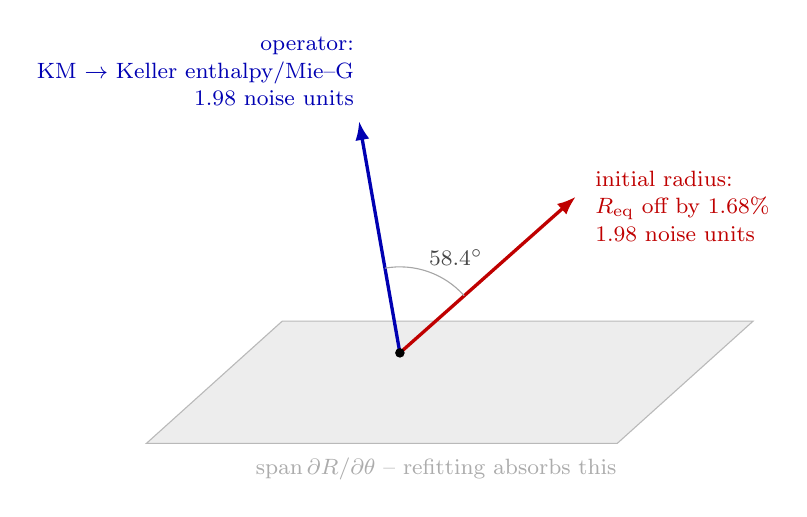
\begin{tikzpicture}[scale=1.15]
  \fill[gray!14] (0.2,0) -- (5.4,0) -- (6.9,1.35) -- (1.7,1.35) -- cycle;
  \draw[gray!55] (0.2,0) -- (5.4,0) -- (6.9,1.35) -- (1.7,1.35) -- cycle;
  \node[gray!65,anchor=north east] at (5.5,-0.05)
    {\footnotesize $\operatorname{span}\partial R/\partial\theta$ -- refitting absorbs this};
  % the two remainders, drawn at the measured 58.4 degrees and the same measured length
  \draw[-{Latex[length=2.4mm]},very thick,blue!70!black] (3,1) -- (2.549,3.560);
  \draw[-{Latex[length=2.4mm]},very thick,red!75!black] (3,1) -- (4.944,2.726);
  \draw[gray!70] (3,1) ++(41.6:0.95) arc (41.6:100:0.95);
  \node[gray!55!black] at (3.62,2.05) {\footnotesize $58.4^\circ$};
  \fill[black] (3,1) circle (1.5pt);
  \node[blue!70!black,anchor=south east,align=right] at (2.6,3.62)
    {\footnotesize operator:\\[-2pt]\footnotesize KM $\to$ Keller enthalpy/Mie--G\\[-2pt]\footnotesize $1.98$ noise units};
  \node[red!75!black,anchor=west,align=left] at (5.05,2.62)
    {\footnotesize initial radius:\\[-2pt]\footnotesize $R_{\mathrm{eq}}$ off by $1.68\%$\\[-2pt]\footnotesize $1.98$ noise units};
\end{tikzpicture}
\caption{The size of the operator result, against the size of an error bar this work set to
zero. Both arrows are what survives refitting the material -- the part of a perturbation that
lies outside the shaded span, and so the only part any experiment can see. They are drawn at
their measured length and their measured separation. A \SI{1.68}{\percent} error in the
inferred equilibrium radius leaves exactly as much residual as replacing the bubble-dynamics
operator does. The \SI{58.4}{\degree} between them is the reason this is a call to fit
$R_{\mathrm{eq}}$ rather than to abandon the ranking: at that angle the two are separable in
principle, and \cref{sec:axes} confirms the initial state absorbs under \SI{5}{\percent} of
the operator difference.}
\label{fig:reqsize}
\end{figure}


\begin{figure}[t]
\centering
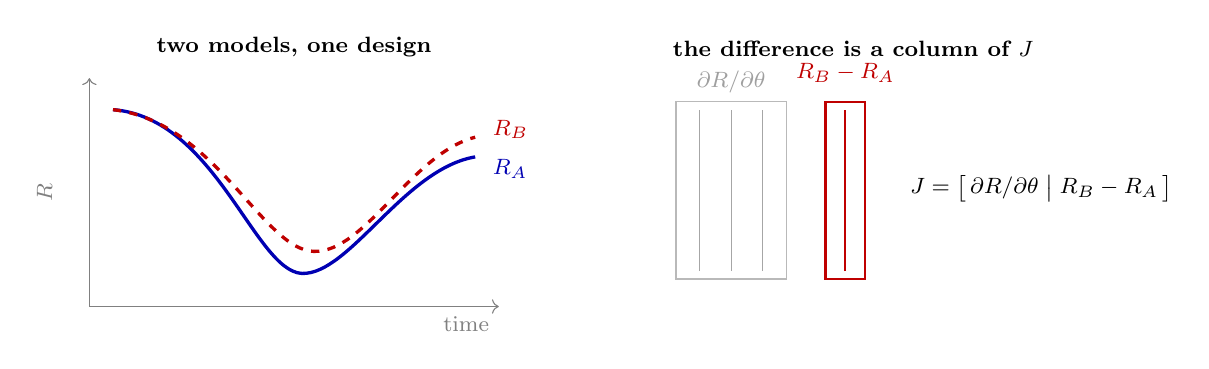
\begin{tikzpicture}[scale=1.0]
\begin{scope}
  \draw[->,gray] (0,0) -- (5.2,0) node[anchor=north east] {\footnotesize time};
  \draw[->,gray] (0,0) -- (0,2.9);
  \node[gray,rotate=90,anchor=south] at (-0.35,1.45) {\footnotesize $R$};
  \draw[blue!70!black,very thick] (0.3,2.5) .. controls (1.6,2.4) and (2.1,0.45) .. (2.7,0.42)
    .. controls (3.3,0.4) and (4.0,1.75) .. (4.9,1.9);
  \draw[red!75!black,very thick,dashed] (0.3,2.5) .. controls (1.6,2.35) and (2.2,0.72) .. (2.85,0.7)
    .. controls (3.5,0.68) and (4.1,1.95) .. (4.9,2.15);
  \node[blue!70!black,anchor=west] at (5.0,1.75) {\footnotesize $R_A$};
  \node[red!75!black,anchor=west] at (5.0,2.25) {\footnotesize $R_B$};
  \node[anchor=south] at (2.6,3.05) {\footnotesize\textbf{two models, one design}};
\end{scope}
\begin{scope}[xshift=7.3cm]
  \node[anchor=south] at (2.4,3.05) {\footnotesize\textbf{the difference is a column of $J$}};
  \draw[gray!55] (0.15,0.35) rectangle (1.55,2.6);
  \node[gray!75] at (0.85,2.85) {\footnotesize $\partial R/\partial\theta$};
  \foreach \x in {0.45,0.85,1.25} { \draw[gray!70] (\x,0.45) -- (\x,2.5); }
  \draw[red!75!black,thick] (2.05,0.35) rectangle (2.55,2.6);
  \draw[red!75!black,thick] (2.3,0.45) -- (2.3,2.5);
  \node[red!75!black,anchor=south] at (2.3,2.72) {\footnotesize $R_B-R_A$};
  \node[anchor=west,align=left] at (3.0,1.5)
    {\footnotesize $J=\big[\,\partial R/\partial\theta \;\big|\; R_B-R_A\,\big]$};
\end{scope}
\end{tikzpicture}
\caption{Turning a model choice into a parameter. Writing
$R(\theta,\varepsilon)=(1-\varepsilon)R_A(\theta)+\varepsilon R_B(\theta)$ gives
$\partial R/\partial\varepsilon = R_B-R_A$ at $\varepsilon=0$, so the difference between two
models becomes one more column of the Jacobian. Discrimination and estimation then live in a
single information matrix, and $D$-optimality over the augmented set balances learning the
material against learning which model produced the trace. Nothing about the criterion changes,
so the certificate still applies. The variance of $\varepsilon$ after the material is fitted
out is what says whether a design can tell the models apart at all.}
\label{fig:augment}
\end{figure}


\begin{figure}[t]
\centering
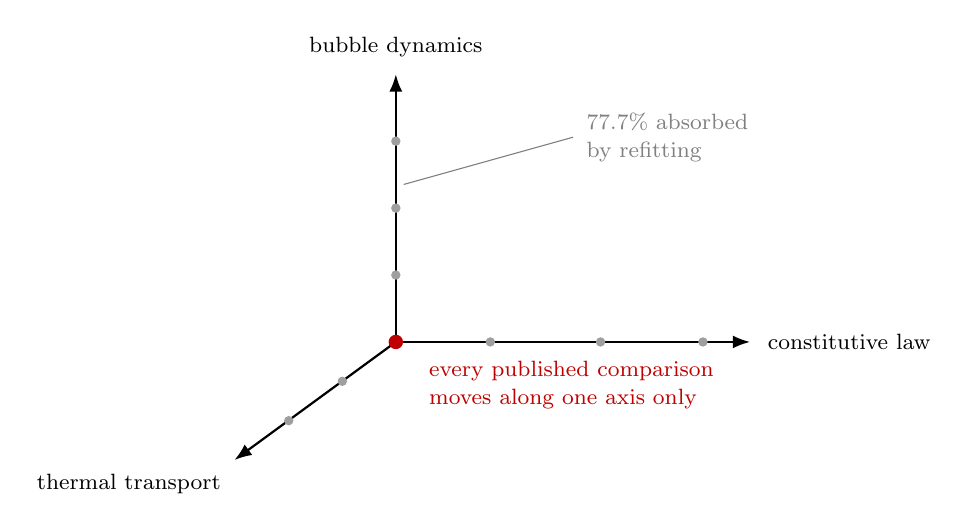
\begin{tikzpicture}[scale=1.0]
  \draw[-{Latex[length=2.2mm]},thick] (0,0) -- (4.5,0);
  \draw[-{Latex[length=2.2mm]},thick] (0,0) -- (0,3.4);
  \draw[-{Latex[length=2.2mm]},thick] (0,0) -- (-2.05,-1.5);
  \node[anchor=west] at (4.6,0) {\footnotesize constitutive law};
  \node[anchor=south] at (0,3.5) {\footnotesize bubble dynamics};
  \node[anchor=north east] at (-2.1,-1.55) {\footnotesize thermal transport};
  \foreach \x/\lab in {1.2/qSLS, 2.6/qSLS2, 3.9/qSLSthin} {
    \fill[gray!75] (\x,0) circle (1.7pt); }
  \foreach \y/\lab in {0.85/{}, 1.7/{}, 2.55/{}} { \fill[gray!75] (0,\y) circle (1.7pt); }
  \fill[gray!75] (-0.68,-0.5) circle (1.7pt);
  \fill[gray!75] (-1.36,-1.0) circle (1.7pt);
  \fill[red!75!black] (0,0) circle (2.6pt);
  \node[red!75!black,anchor=west,align=left] at (0.3,-0.55)
    {\footnotesize every published comparison\\[-2pt]\footnotesize moves along one axis only};
  \node[gray,anchor=west,align=left] at (2.3,2.6)
    {\footnotesize $77.7\%$ absorbed\\[-2pt]\footnotesize by refitting};
  \draw[gray] (2.25,2.6) -- (0.1,2.0);
\end{tikzpicture}
\caption{Three choices go into every prediction, and they are made independently: the
constitutive law, the bubble-dynamics equation, and whether heat transfer is modeled.
Published comparisons vary the first and leave the other two at the origin. Some of each
change can be canceled by refitting stiffness and viscosity, which makes it invisible no
matter how the experiment is run; what remains is $22\%$ of an operator change, $57\%$ of a
constitutive change and $53\%$ of a thermal one, and no two of those remainders point in
similar directions. All three are therefore distinguishable in principle.}
\label{fig:modelspace}
\end{figure}

\section{Separability of the model axes}
\label{sec:axes}

With the constitutive law, the operator and the thermal treatment all uncertain, the question
is not which experiment discriminates but whether the axes are separable at all. They need not
be, in two ways. A difference lying in the span of $\partial R/\partial\theta$ is reproduced by
refitting the material, and is then invisible at every design (\cref{fig:absorption}). And two
axes whose remainders are nearly parallel move the evidence together, so no design can say
which moved it.

\begin{center}
\begin{tabular}{lcccc}
\toprule
axis & size & after refit & absorbed & \,+\,initial state \\
\midrule
dynamics (KM $\to$ Keller enthalpy/Mie--G) & 8.89 & \textbf{1.98} & \textbf{77.7\%} & 1.89 \\
constitutive (one $\to$ two modes) & 14.42 & 8.14 & 43.5\% & 7.72 \\
thermal (cold $\to$ bubble\,+\,medium) & \textbf{15.99} & 8.46 & 47.1\% & 7.80 \\
\bottomrule
\end{tabular}
\end{center}

\noindent in units of the record's noise. The last column widens the refit span to include
$R_0$ and $R_{\mathrm{eq}}$, which are held at their measured values everywhere else in this
work. They take a further $4.7$, $5.2$ and \SI{7.8}{\percent} of what the material left, so
none of these differences is initial-state freedom in disguise. A near-zero number here is
also what a broken projection would report, so the operation is checked both ways on the same
vectors: handed the difference itself the basis absorbs it to $5\times10^{-15}$, handed a
random column it absorbs $0.02$ of $1.98$.

The remainders sit at $46$, $71$ and \SI{38}{\degree} to one another. No pair is confounded,
so the design problem is well posed for all three. Two things follow that were not expected.

Thermal is the \emph{largest} lever, not a negligible one. It moves the trace most and
survives refitting most. So the earlier observation -- that switching it on made $\chi^2/N$
slightly worse -- says the direction it moves in is not the one the record wants, not that it
is small.

The operator is the most absorbed axis by a wide margin. That is the mechanism behind
\cref{sec:operator}: most of an operator change can be mimicked by adjusting the material.

\paragraph{A design against all three.} Make each axis a parameter through
$R(\theta,\varepsilon)=(1-\varepsilon)R_A+\varepsilon R_B$, so $\partial R/\partial\varepsilon =
R_B-R_A$ is one more column of $J$. This puts discrimination and estimation in one information
matrix and leaves the criterion concave, so the certificate of
\cref{fig:certificate-schematic} applies unchanged. The information is averaged over a
decade of $g\alpha$, because operator information is governed by collapse depth and a measure
certified at one material misranks others. The measure certifies at a gap of $10^{-9}$ on four
support points.

\begin{center}
\begin{tabular}{lccc}
\toprule
axis & variance at the optimum & at the \SI{15}{\celsius} geometry & efficiency \\
\midrule
dynamics & $6.78\times10^{-3}$ (binding) & $9.91\times10^{-3}$ & $68.4\%$ \\
constitutive & $5.45\times10^{-4}$ & $2.24\times10^{-2}$ & $2.4\%$ \\
thermal & $4.40\times10^{-4}$ & $1.05\times10^{-2}$ & $4.2\%$ \\
\bottomrule
\end{tabular}
\end{center}

\noindent Reported per axis rather than as one determinant. A design maximizing $\det$ could
buy its whole score on the two easy axes and leave the operator undetermined without saying
so. The experiments performed are near-best for the hardest axis and $24$ to $41$ times off for
the two easiest. So a change of geometry buys a great deal of constitutive and thermal
discrimination at little cost to the operator. The support wants $R_{\max}$ near
\SI{60}{\micro\metre} at high stretch and near \SI{1200}{\micro\metre} at low stretch, against
the \SI{277}{\micro\metre} and stretch $7.09$ performed.

\section{Fitting the initial radius}
\label{sec:reqprior}

\Cref{sec:operator} reports operator margins of a few nats while holding $R_{\mathrm{eq}}$
fixed, and a \SI{1.68}{\percent} error in $R_{\mathrm{eq}}$ is worth as much as the operator
change those margins measure. A quantity that large cannot be asserted. So we fit it, as a
nuisance parameter with a prior. The question is not whether the evidence moves -- adding a
parameter always moves it -- but whether the \emph{ordering} does. An operator preferred by $17$ nats
with $R_{\mathrm{eq}}$ pinned, and not preferred once it floats, was never an operator result.

The prior width is the whole argument, and nothing measures it. Too wide and $R_{\mathrm{eq}}$ absorbs the operator difference, which reads as ``the
operators are indistinguishable'' while being a statement about the box. Too narrow and the
pinned answer is reproduced by construction. We therefore sweep the half-width over
$\SIrange{3}{25}{\percent}$ rather than choose one. A conclusion that holds across that range
is a conclusion; one that flips inside it is a prior.

\paragraph{A convergence gate with no tuning constant.} Every wider box contains every
narrower one, and all of them contain $R_{\mathrm{eq}}$ at its inferred value, which is the
pinned fit. The best attainable $\chi^2/N$ can therefore only fall as the width grows. A cell
that rises has not found its own optimum. This matters because it caught a real failure: at
ten multistart restarts, five of $72$ cells failed it, one reporting $-117$ nats between a
$+13$ and a $+7$ -- which reads as a prior effect and is a search that stopped early. At $24$
restarts two cells fail, and both are excluded below rather than read as physics.

\begin{center}
\begin{tabular}{lcccccc}
\toprule
& \multicolumn{2}{c}{\SI{15}{\celsius}} & \multicolumn{2}{c}{\SI{23}{\celsius}}
& \multicolumn{2}{c}{\SI{33}{\celsius}} \\
\cmidrule(lr){2-3}\cmidrule(lr){4-5}\cmidrule(lr){6-7}
operator & pinned & $\pm25\%$ & pinned & $\pm25\%$ & pinned & $\pm25\%$ \\
\midrule
Rayleigh--Plesset & $-165.0$ & $\mathbf{-178.6}$ & $-76.9$ & $\mathbf{-81.8}$ & $-74.4$ & $\mathbf{-74.2}$ \\
Keller--Miksis & $0$ & $0$ & $0$ & $0$ & $0$ & $0$ \\
Keller enthalpy/Tait & $+6.1$ & $+0.8$ & $+2.1$ & $+0.1$ & $+0.8$ & $+0.8$ \\
Gilmore/Tait & $+18.5$ & $\mathbf{+5.0}$ & $+4.3$ & $+0.5$ & $+1.9$ & $-0.0$ \\
Keller enthalpy/Mie--G & $+4.7$ & $+0.3$ & $+1.6$ & $+0.1$ & $+0.6$ & $+0.9$ \\
Gilmore/Mie--G & $+20.7$ & $\mathbf{+11.2}$ & $+4.3$ & --- & $+1.1$ & $-0.3$ \\
\bottomrule
\end{tabular}
\end{center}

\noindent nats against Keller--Miksis; ``---'' marks the one cell the gate excluded. Of $17$
orderings the pinned fit called decisive, $15$ stay decisive and keep their sign at every
width. None reverses. Two fall below five nats at some width, both at \SI{15}{\celsius}.

The conclusions of \cref{sec:operator} therefore survive, but not equally. \emph{Compressibility
is required} at every width and on every record, by $74$ to $179$ nats -- the most robust
statement in this work. \emph{Gilmore beats the pressure form} at \SI{15}{\celsius}, still by
$5$ to $11$ nats with $R_{\mathrm{eq}}$ free. But at \SI{23}{\celsius} and \SI{33}{\celsius}
every margin above Keller--Miksis collapses to under a nat. Those two records never had
operator discrimination; pinning $R_{\mathrm{eq}}$ is what made it look as though they did.

\paragraph{The data want a larger equilibrium radius.} The fitted scale is the same story
told forwards, and it is the most consistent number in this study. At $\pm3\%$ every one of
the $18$ cells pins against the upper edge. Given room, they agree closely: $1.104$ to
$1.115$ at \SI{15}{\celsius}, $1.074$ to $1.086$ at \SI{23}{\celsius}, and $1.032$ to $1.040$
at \SI{33}{\celsius}, across six operators and two prior widths.

So $R_{\mathrm{eq}}$ is inferred about \SIrange{3}{11}{\percent} too small, and the fit says
so whichever operator it is asked through. The residual improves accordingly --- $\chi^2/N$
falls from $0.97$ to $0.62$ at \SI{15}{\celsius}, $1.03$ to $0.90$ at \SI{23}{\celsius}, and
$0.44$ to $0.38$ at \SI{33}{\celsius}. That the offset shrinks as the gel warms is a pattern
we can measure but not yet explain, and it is larger than the \SI{1.68}{\percent} that makes
$R_{\mathrm{eq}}$ worth as much as the operator choice.

\section{Scoring the thermal treatment, and failing to}
\label{sec:thermal}

\Cref{sec:axes} finds the thermal treatment the largest of the three model axes: it moves the
trace by $16$ noise units and keeps $8.5$ after the material absorbs what it can. It is also
the only one never scored. The one number in circulation is a $\chi^2/N$ that got slightly
worse when heat transfer was switched on, which is a fit statistic and not evidence.

Scoring it means running the same comparison as \cref{sec:operator} with the thermal
treatment varied and the material axes held identical, so the Occam terms cancel and the
difference is a Bayes factor between physics. We report the attempt because it did not work,
and because how it failed is worth knowing.

\begin{center}
\begin{tabular}{lccc}
\toprule
record & cold & bubble & bubble\,+\,medium \\
\midrule
\SI{15}{\celsius} & $0$ & $-6.4$ & $+21.6$ \\
\SI{23}{\celsius} & $0$ & $\mathbf{+2.6}$ & $\mathbf{+8.0}$ \\
\SI{33}{\celsius} & $0$ & $-5.7$ & $-66.0$ \\
\bottomrule
\end{tabular}
\end{center}

\noindent nats against the cold model, at $24$ multistart restarts. Only the middle row may
be read. Repeating the study at ten restarts and again at $24$ -- a $2.4\times$ change of
budget -- moves the \SI{23}{\celsius} rows by $0.00$, $0.00$ and $0.01$ nats, and the others
by $15$, $153$, $19$ and $68$. The cold baselines are stable everywhere, so the record and
the material are not at fault; the thermal likelihood surface is.

The decisive detail is that \emph{more restarts fitted worse}. At \SI{15}{\celsius} the bubble
treatment reached $\chi^2/N = 0.895$ from ten starts and $1.039$ from twenty-four; at
\SI{33}{\celsius} bubble\,+\,medium went from $0.428$ to $1.073$. Best-of-$24$ cannot be worse
than best-of-$10$ at a converged optimum, so the search is landing in different basins rather
than refining one. A third increase of the budget is therefore not the remedy, and this is the
third budget tried.

What this does and does not say. It does not say the thermal treatment is unsupported: on the
one record where the fit converges, both treatments are favored, bubble\,+\,medium by $8$
nats. It says that scoring thermal physics by multistart least squares does not work on these
records, and that the fix is a better search -- warm-starting each thermal fit from the
converged cold optimum, rather than sampling a four-dimensional box afresh. Until then the
\SI{15}{\celsius} and \SI{33}{\celsius} rows above are search noise, and we decline to read
the sign of either.

\section{Experimental design}
\label{sec:design}

\subsection*{Designing without assuming the model}

Everything above optimizes the Fisher information of one model at its fitted parameters,
which is circular if that model is wrong. Two checks that do not privilege it.

\paragraph{The record is information-rich; the parameterization is not.}
Draw $400$ trajectories from the posterior and take the singular values of the centered
ensemble. Eleven modes clear the trial noise floor of $0.018\,R_{\max}$. That is not a count
of identifiable combinations: four parameters span at most a four-dimensional manifold, and
the extra modes are its curvature. But the record distinguishes far more shapes than the fit
extracts. The limit is qSLS, not the measurement.

\paragraph{Discrimination does not privilege a model.}
T-optimality \citep{atkinson1975design} asks a different question: which design makes the
candidates disagree most? The criterion is
%
\begin{equation}
T(d) \;=\; \min_{\theta_2} \; \bigl\lVert m_1(\hat\theta_1, d) - m_2(\theta_2, d) \bigr\rVert / \sigma ,
\label{eq:topt}
\end{equation}
%
and the minimization is the whole content of it. A rival that retunes its parameters to
imitate has not been discriminated against. So the separation is measured against the rival's
\emph{best imitation}, never against its own fitted values.

Two errors here inflated $T$, both for one structural reason. $T$ is a \emph{minimum}, so
anything stopping short of it reports discrimination that is not there. Evaluating each rival
at its own fit gave $2.69$ for qSLS--SLS at the present design; re-fitting with one
Nelder--Mead pass gave $0.67$.

Restarting and polishing changed other entries again. At $1200\,\mu$m the reported $4.92$
fell to $2.38$. A $0.1\%$ change of design moved one loose evaluation from $7.25$ to $1.36$
-- the optimizer's signature, not the physics. The converged values are:

\begin{center}
\begin{tabular}{lccc}
\toprule
design & qSLS--SLS & qSLS--qKV & qSLS--NHKV \\
\midrule
$277\,\mu$m, stretch $7.09$ (present) & $0.67$ & $4.53$ & $4.37$ \\
$277\,\mu$m, stretch $5.00$ & $0.72$ & $4.61$ & $4.61$ \\
$277\,\mu$m, stretch $3.00$ & $0.74$ & $1.72$ & $1.72$ \\
$199\,\mu$m, stretch $3.55$ (E-optimal) & $0.56$ & $2.59$ & $2.59$ \\
$895\,\mu$m, stretch $4.93$ & $\mathbf{2.39}$ & $7.13$ & $\mathbf{7.13}$ \\
$910\,\mu$m, stretch $5.19$ & $1.36$ & $6.97$ & $6.97$ \\
$1200\,\mu$m, stretch $7.09$ & $2.38$ & $5.03$ & $5.63$ \\
$100\,\mu$m, stretch $20.0$ & $1.26$ & $\mathbf{8.04}$ & $4.17$ \\
$57\,\mu$m, stretch $19.5$ & $1.64$ & $5.53$ & $5.00$ \\
\bottomrule
\end{tabular}
\end{center}

At the present design SLS imitates qSLS to within $0.67$ noise units, inside the measurement
scatter. An unrelated calculation corroborates it. A systematic offset of $0.668\sigma$ over
$201$ samples contributes $201 \times 0.668^2 = 89.7$ to $\chi^2$, against a measured
log-evidence gap of $101.6$. Two computations sharing no machinery, agreeing to $12\%$.

\paragraph{These values are upper bounds, and the criterion is the reason.}
$T$ is an inner \emph{global} minimization, and that minimization is multimodal.
Nelder--Mead and Gauss--Newton both converge, to different basins. At $895\,\mu$m
Nelder--Mead returns $2.39$ against Gauss--Newton's $1.52$; at $1200\,\mu$m the ordering
reverses.

Multistart Gauss--Newton finds a lower value in $12$ of $27$ cells. Analytic Jacobians make
it $44\times$ cheaper than the derivative-free version -- $34$\,s against $25$ minutes for
the table. A stationarity check from the same Jacobians reports $11$ cells still not at a
minimum.

Every improvement to the optimizer lowers the scores, because a better-optimized rival
imitates better. So the tabulated values are upper bounds on discrimination. The true
separations are smaller than any of them.

This is not a defect of the implementation but of the criterion. A minimum is attained at a
point, so landing in the wrong basin gives a wrong answer with no indication that anything
went wrong, and enumerating the outer design space exactly does not repair it: a dense grid
over an unreliable integrand produces a front that is precisely wrong. Any criterion built
on an argmin -- $T$-optimality, profile likelihood, minimax design -- inherits this.

The structural fix is to replace the minimum with an integral. Treating the model label as a
discrete parameter makes discrimination an expected-information-gain problem over the
augmented parameter $(\theta, m)$, whose inner quantity is the marginal likelihood
$\int p(Y\mid\theta,M,d)\,\pi(\theta\mid M)\,\mathrm d\theta$. An integral accumulates over
all modes instead of requiring the best one be found. Multimodality stops being a failure mode
and becomes a property of the integrand: a missed mode biases the evidence slightly rather
than corrupting the criterion.

It also puts discrimination and parameter precision in one framework. The cost is that the
marginal likelihood is prior-sensitive where $T$ is not. The prior becomes part of the
criterion rather than a nuisance.

\paragraph{The criteria do not agree.}
Computed correctly, the criteria want different experiments. E-optimality peaks at $199\,\mu$m and stretch $3.55$. Separating qSLS from SLS or from NHKV is
best at $895\,\mu$m and stretch $4.93$. Separating qSLS from qKV is best at $100\,\mu$m and
stretch $20$, near the opposite corner of the design space. At the E-optimal design the
discrimination scores are the worst in the table, so the conflict is not marginal.

The reason is physical, not numerical. Telling a material with a relaxation mode from one
without needs a collapse fast enough to excite it. Separating $g$ from $\alpha$ needs a gentle
collapse, because the term of $Z_e$ carrying that distinction dies as $\lambda^{-4}$. No design
is both fast and gentle.

There is accordingly no single best design, and a scalar design objective is answering a
question that has no scalar answer. What replaces it is the \emph{Pareto front}: the set of
designs on which no other design is better on every criterion at once. Enumerating a
$14\times18$ grid over $(R_{\max}, \lambda)$ and applying that test leaves $12$ designs
undominated, spanning $50$--$1200\,\mu$m and stretch $4$--$18$. Reporting that set rather than
a single optimum is the honest summary of an experiment serving several questions at once;
\texttt{pyimr.pareto.explore\_tradeoff} computes it.

The $T$ columns entering the domination test are upper bounds, so the front is provisional in
its discrimination coordinates. The E-optimality coordinate is an eigenvalue of
$J^{\mathsf T}J$ with no inner optimization, and carries no such reservation.

\subsection*{Discrimination as an integral rather than a minimum}
\label{sec:integral}

Everything above scores a design by $T$, defined through a \emph{global minimum} over the
rival's parameters. That definition is the trouble in the previous subsection, and the trouble
is structural rather than computational. Here we replace the minimum with an integral, say why
that is more robust, and report what it gives.

\paragraph{The model label is a parameter.}
Write $M \in \{M_1, M_2\}$ for the model index with prior $p(M)$, and let each model carry
its own parameter $\theta$ with prior $\pi(\theta \mid M)$. Nothing distinguishes $M$ from
any other unknown, so the information a design $d$ yields about it is the mutual information
%
\begin{equation}
I(M; Y \mid d)
= \mathbb{E}_{M}\,\mathbb{E}_{Y \mid M, d}
  \left[\log \frac{p(Y \mid M, d)}{p(Y \mid d)}\right],
\qquad
p(Y \mid d) = \sum_{M} p(M)\, p(Y \mid M, d),
\label{eq:model-mi}
\end{equation}
%
the expected reduction in entropy of $M$ -- exactly as the expected information gain above is
the expected reduction in entropy of $\theta$. Discrimination and estimation are one criterion
applied to different components of the augmented unknown $(\theta, M)$. They are not competing
philosophies: the earlier tension between $T$- and $E$-optimality is about \emph{which
component we care about}, not about two schools.

The quantity entering~\eqref{eq:model-mi} is the marginal likelihood, or evidence,
%
\begin{equation}
p(Y \mid M, d) = \int p(Y \mid \theta, M, d)\, \pi(\theta \mid M)\, \mathrm{d}\theta ,
\label{eq:model-evidence}
\end{equation}
%
the same object as~\eqref{eq:evidence} but now at a hypothetical design and for hypothetical
data. It is an integral over $\theta$, and that single fact is what the rest of this
subsection turns on.

\paragraph{The criterion actually computed.}
Rather than~\eqref{eq:model-mi} we score a design by the expected log Bayes factor in favor
of the model that generated the data,
%
\begin{equation}
U(d)
= \mathbb{E}_{Y \sim p(\cdot \mid M_1, d)}
  \left[\log p(Y \mid M_1, d) - \log p(Y \mid M_2, d)\right]
= D_{\mathrm{KL}}\!\left(p(\cdot \mid M_1, d)\,\|\,p(\cdot \mid M_2, d)\right).
\label{eq:elbf}
\end{equation}
%
Recognizing it as a Kullback--Leibler divergence between the two prior-predictive
distributions settles its properties. By Gibbs' inequality $U(d) \ge 0$, with equality exactly
when the two predictives agree almost everywhere: \emph{a model cannot discriminate against
itself, at any design}.

That is sharp and falsifiable, and it is what the implementation is tested against. Two
independently drawn banks from one family must score zero; any systematic excess is bias.

Equation~\eqref{eq:model-mi} relates by
$I(M;Y\mid d) = \tfrac12[D_{\mathrm{KL}}(p_1\|\bar p) + D_{\mathrm{KL}}(p_2\|\bar p)]$ with
$\bar p$ the equal mixture. So~\eqref{eq:elbf} is the same comparison read against the rival
rather than the mixture -- the more direct statement of ``how strongly will this experiment
favor the truth''.

\paragraph{Why an integral is robust where a minimum is not.}
Both criteria require an inner computation that can go wrong. The asymmetry is in how the
error propagates.

For $T$, any optimizer returns $\hat T = \lVert m_1 - m_2(\hat\theta_2)\rVert/\sigma$ at
whatever point it stopped, and since $T$ is a minimum, $\hat T \ge T$ always. If $\hat\theta_2$
lies in the correct basin but is imprecise, stationarity gives
$\hat T - T = O(\lVert\hat\theta_2 - \theta_2^\star\rVert^2)$ and the error is negligible. If
it lies in the \emph{wrong basin}, the error is $O(1)$: a fixed, unbounded overstatement with
nothing in the returned value to indicate it. This is what was measured -- Nelder--Mead and
Gauss--Newton returning $2.39$ and $1.52$ at one design and reversing at another.

For the evidence, suppose the posterior has modes $k = 1,\dots,K$ contributing
$Z = \sum_k Z_k$, and a procedure finds only a subset $\mathcal{S}$. Then
%
\begin{equation}
\log \hat Z - \log Z
= \log\!\left(1 - \sum_{k \notin \mathcal{S}} \frac{Z_k}{Z}\right),
\label{eq:mode-loss}
\end{equation}
%
so the error is controlled by the \emph{posterior weight} of what was missed. Missing a
subdominant mode costs $O(Z_k/Z)$ and missing a negligible one costs nothing. Because the
contributions add, a multistart that finds several modes can sum them rather than choose
between them, and each additional mode found monotonically improves the estimate. There is no
analogue for a minimum, where finding more candidates only ever changes which single one is
reported.

This is the whole argument for the change, and it is worth stating plainly: multimodality is
a \emph{failure mode} for a minimum and merely a \emph{property of the integrand} for an
integral.

\paragraph{Estimating the evidence I: prior sampling, and why it fails here.}
The direct estimator draws $\theta_s \sim \pi(\theta \mid M)$ and averages the likelihood,
%
\begin{equation}
\hat Z = \frac{1}{S}\sum_{s=1}^{S} p(Y \mid \theta_s, M, d),
\qquad
w_s = p(Y \mid \theta_s, M, d),
\label{eq:prior-mc}
\end{equation}
%
which is unbiased for $Z$, though $\log \hat Z$ is biased low by Jensen's inequality. Its
reliability rides on the spread of the weights, summarized by the effective sample size
%
\begin{equation}
S_{\mathrm{eff}} = \frac{\left(\sum_s w_s\right)^2}{\sum_s w_s^2}
\;\in\; [1, S],
\label{eq:ess-evidence}
\end{equation}
%
which equals $S$ when all draws contribute equally and $1$ when a single draw dominates. It
costs nothing to compute. It is also the only thing standing between this estimator and a
confidently reported number with no content.

That it must fail here can be seen in advance. With $N$ samples the log-likelihood scales as
$\log p(Y\mid\theta) \simeq -\tfrac12 N \bar d(\theta)$ for a mean squared discrepancy
$\bar d$, so weights are $w_s \propto \exp[-\tfrac12 N \bar d(\theta_s)]$ and the ratio of the
two largest is exponential in $N$. Useful draws are those landing inside the posterior. Its
width is $O(N^{-1/2})$ in each of $p$ directions, so the expected number of useful draws is
%
\begin{equation}
\mathbb{E}[\#\text{useful}] \;\sim\; S \cdot \frac{\mathrm{vol}(\text{posterior})}
{\mathrm{vol}(\text{prior})} \;\sim\; S\,N^{-p/2}.
\label{eq:useful-draws}
\end{equation}
%
For the present study $N = 201$, $p = 4$ and $S = 220$, giving
$220 \times 201^{-2} \approx 5 \times 10^{-3}$ -- fewer than one useful draw.

The measurement agrees exactly. $S_{\mathrm{eff}} = 1.0$ at \emph{every} design tried, with
reported values between $793$ and $10\,979$ nats that are pure noise. The standard errors ran
$56$ to $130$ throughout and looked entirely respectable. Without~\eqref{eq:ess-evidence} the
failure is invisible.

\paragraph{Estimating the evidence II: Laplace.}
Expand $\log[p(Y\mid\theta)\pi(\theta)]$ to second order about its maximum $\hat\theta$ and do
the resulting Gaussian integral. As in~\eqref{eq:laplace},
%
\begin{equation}
\log Z \simeq \log p(Y \mid \hat\theta)
 + \log \pi(\hat\theta)
 + \tfrac{p}{2}\log 2\pi
 - \tfrac12 \log \det H ,
\qquad
H = -\nabla^2 \log p(Y\mid\theta)\big|_{\hat\theta}.
\label{eq:laplace-evidence}
\end{equation}
%
For Gaussian data $H = J^{\mathsf T}J + \sum_i r_i \nabla^2 r_i$. Dropping the second term --
the Gauss--Newton approximation, valid when residuals are small or the model nearly linear --
leaves $H \simeq J^{\mathsf T}J$, which the fit already computed. Parameterizing so the prior is
uniform on the unit cube makes $\pi(\hat\theta) = 1$, and with whitened residuals
$r = (m - y)/\sigma$,
%
\begin{equation}
\log Z \simeq
-\tfrac12 \lVert r \rVert^2
-\tfrac{N}{2}\log\!\left(2\pi\sigma^2\right)
+\tfrac{p}{2}\log 2\pi
-\tfrac12 \log \det\!\left(J^{\mathsf T}J\right).
\label{eq:laplace-unit}
\end{equation}
%
The first two terms are the best fit; the last two are the Occam factor, and their sign is
what prevents a more flexible model from winning on fit alone. Crucially
for the present purpose, \eqref{eq:laplace-unit} does not care how sharp the likelihood is,
which is precisely the regime that destroyed~\eqref{eq:prior-mc}. It is affordable only
because the fit uses analytic Jacobians: derivative-free minimization of the same objective
costs $55$\,s against $7.6$\,s, and the Jacobian needed for $\det(J^{\mathsf T}J)$ is a
by-product of the solve rather than an extra cost.

\paragraph{The two criteria are consistent where both can be computed.}
The criteria are not independent, and the relation between them is a check on both. If the
true model fits to within noise, $\chi^2_1 \approx N$, while a rival that cannot fit leaves a
residual of root-mean-square $T\sigma$, so $\chi^2_2 \approx N T^2$. Substituting into the
leading term of~\eqref{eq:laplace-unit},
%
\begin{equation}
\log \mathrm{BF} \;\approx\; \tfrac12\left(\chi^2_2 - \chi^2_1\right)
\;\approx\; \tfrac{N}{2}\left(T^2 - 1\right)
\;\xrightarrow{\;T \gg 1\;}\; \tfrac{N}{2}T^2 ,
\label{eq:t-to-bf}
\end{equation}
%
up to the Occam terms, which $T$ has no way to express. Testing~\eqref{eq:t-to-bf} against
the measured values:

\begin{center}
\begin{tabular}{lccc}
\toprule
design & $T$ (vs SLS) & $\tfrac{N}{2}T^2$ predicted & measured $U$ (nats) \\
\midrule
$199\,\mu$m, stretch $3.55$ & $0.56$ & $31.5$ & $35.4 \pm 12.2$ \\
$895\,\mu$m, stretch $4.93$ & $1.52$ & $232$ & $150 \pm 73$ \\
\bottomrule
\end{tabular}
\end{center}

Two computations sharing no machinery -- one a constrained least-squares minimum, the other
a marginal likelihood by Laplace -- agreeing to within their stated uncertainty. The residual
gap at $895\,\mu$m is of the right sign and size for the Occam penalty that qSLS pays for its
fourth parameter.

\paragraph{What it costs, and where it is not yet trustworthy.}
Two prices are paid for removing the minimum, and both are real.

\emph{Prior sensitivity.} $Z$ depends on $\pi(\theta\mid M)$ through the normalization
of~\eqref{eq:model-evidence}. Widening a prior by a factor $c$ in each of $p$ directions
divides the evidence by roughly $c^{p}$ without changing the fit at all. This is the
Lindley--Jeffreys effect~\citep{lindley1957statistical,jeffreys1935some}, and it is not a
defect to engineer away: a model whose prior is diffuse really is less supported by data that
pin it down.

But it makes the prior part of the criterion, where $T$ needed none, so the prior must be
stated. Centering each rival's prior on its fit to the \emph{existing} record produced a
criterion measuring prior placement instead of discriminability, with every Laplace expansion
invalid. The results here use the wide, physically motivated box of the model-selection grid,
identical across models on every shared parameter.

\emph{Boundary pinning.} Equation~\eqref{eq:laplace-evidence} presumes an interior maximum. In
$50$--$90\%$ of the fits at each design the rival's best parameters lie on a face of the prior
box, where the expansion does not apply and the value is not to be trusted.

That it happens is itself informative. A rival that can imitate qSLS only by driving a
parameter to the edge of physical plausibility has, in a meaningful sense, been discriminated
against. But saying so needs a criterion built for a constrained maximum, not a quadratic
expansion about an interior one. Which parameter pins, and whether the pinning is physical or
an artifact of the box, is the outstanding step.

The honest summary: the integral criterion is better founded than $T$ and not yet more
reliable on this problem. The multimodality that made $T$ untrustworthy is genuinely gone.
What replaces it is a dependence on the prior -- now explicit rather than hidden -- and a
boundary condition the current estimator does not handle.

\subsection*{Which criterion the conflict is between}

The scaling argument of \cref{sec:criteria} says a design change that merely amplifies signal
leaves the condition number $\kappa$ untouched. Degeneracy is a property of the eigenvectors,
and only a design that rotates them can remove it.

For these records, E-optimality preferred a larger bubble ($895\,\mu$m,
$\lambda_{\min} = 12.8$). Conditioning and eigenvector composition preferred a gentler collapse
at the present size ($277\,\mu$m at stretch $5$, $\kappa = 4.2\times10^3$, the
modulus--stiffening share of the worst direction falling from $87\%$ to $66\%$). Both are
correct answers to different questions, and \eqref{eq:separability} says which one matters
here.

So there are two distinct disagreements in play, and they have different resolutions. The
classical criteria disagree among themselves because they summarize one spectrum
differently; that is a choice about what one wants to learn. Estimation and discrimination
disagree because they are about different quantities altogether. The next subsection
resolves the second, and in doing so dissolves the first.


\begin{figure}[t]
\centering
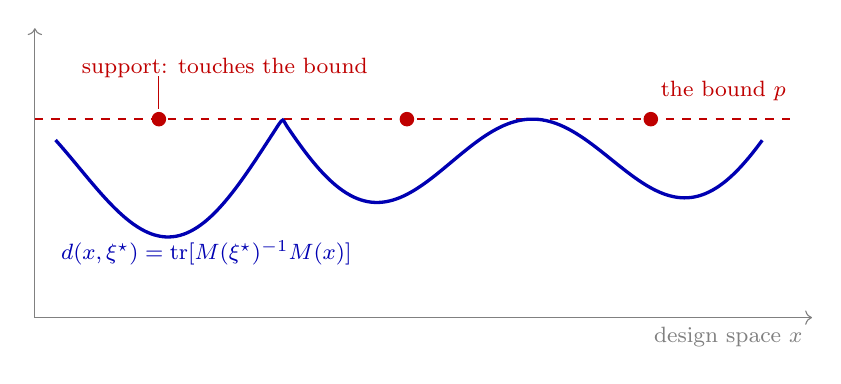
\begin{tikzpicture}[scale=1.05]
  \draw[->,gray] (0,0) -- (9.4,0) node[anchor=north east] {\footnotesize design space $x$};
  \draw[->,gray] (0,0) -- (0,3.5);
  \draw[red!75!black,thick,dashed] (0,2.4) -- (9.2,2.4);
  \draw[blue!70!black,very thick,smooth,samples=200,domain=0.25:8.8]
    plot (\x, {2.4 - 1.5*abs(sin(deg(\x*1.05)))*abs(sin(deg(\x*0.42+0.6)))});
  \foreach \x in {1.5, 4.5, 7.45} { \fill[red!75!black] (\x,2.4) circle (2.5pt); }
  \node[red!75!black,anchor=south east] at (9.2,2.5) {\footnotesize the bound $p$};
  \node[blue!70!black,anchor=north west] at (0.2,1.05) {\footnotesize $d(x,\xi^\star)=\operatorname{tr}[M(\xi^\star)^{-1}M(x)]$};
  % one leader only: three fanned out across the panel and ran through the bound label
  \node[red!75!black,anchor=west] at (0.45,3.02) {\footnotesize support: touches the bound};
  \draw[red!75!black,thin] (1.5,2.92) -- (1.5,2.52);
\end{tikzpicture}
\caption{The certificate, which is what makes an optimal design a proof rather than a stopping
rule. Kiefer and Wolfowitz: a measure $\xi^\star$ is $D$-optimal \emph{if and only if} its
sensitivity $d(x,\xi^\star)$ never exceeds the parameter count $p$ anywhere in the design
space, and attains $p$ exactly on the points carrying weight. Both halves are visible at once
-- a curve capped by a level it touches and never crosses -- so a search reports not merely
that it stopped improving but that there is nowhere left for a better design to hide. The gap
$\max_x d(x,\xi^\star)-p$ is the proof's residue; $10^{-9}$ in the designs here.}
\label{fig:certificate-schematic}
\end{figure}


\begin{figure}[t]
\centering
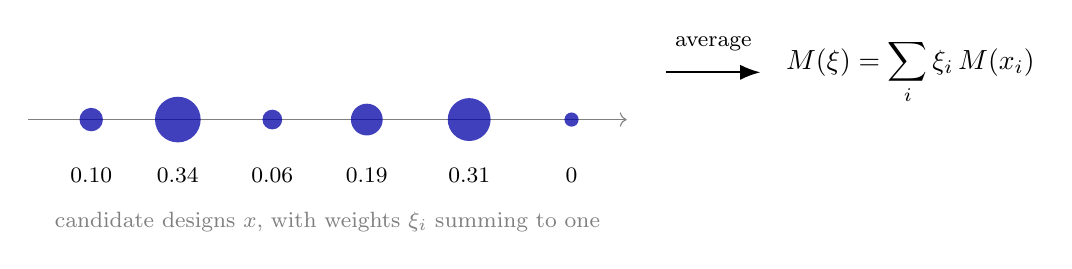
\begin{tikzpicture}[scale=1.0]
  \draw[->,gray] (0,0) -- (7.6,0);
  \foreach \x/\w in {0.8/0.10, 1.9/0.34, 3.1/0.06, 4.3/0.19, 5.6/0.31, 6.9/0.00} {
    \fill[blue!65!black,opacity=0.75] (\x,0) circle ({0.09 + 2.1*\w*0.28});
  }
  \node[anchor=north] at (0.8,-0.5) {\footnotesize $0.10$};
  \node[anchor=north] at (1.9,-0.5) {\footnotesize $0.34$};
  \node[anchor=north] at (3.1,-0.5) {\footnotesize $0.06$};
  \node[anchor=north] at (4.3,-0.5) {\footnotesize $0.19$};
  \node[anchor=north] at (5.6,-0.5) {\footnotesize $0.31$};
  \node[anchor=north] at (6.9,-0.5) {\footnotesize $0$};
  \node[gray,anchor=north] at (3.8,-1.05) {\footnotesize candidate designs $x$, with weights $\xi_i$ summing to one};
  \draw[-{Latex[length=2.6mm]},thick] (8.1,0.6) -- (9.3,0.6);
  \node[anchor=south] at (8.7,0.75) {\footnotesize average};
  \node[anchor=west] at (9.5,0.6)
    {$M(\xi)=\displaystyle\sum_i \xi_i\, M(x_i)$};
\end{tikzpicture}
\caption{A design is a measure, not a point. Each candidate $x_i$ carries an information
matrix $M(x_i)$, and a design assigns weights $\xi_i$ summing to one, read as the fraction of
runs spent at that candidate. The averaged information $M(\xi)$ is linear in $\xi$, so any
concave function of it is concave in the design, and the maximization becomes convex. That
convexity is what makes \cref{fig:certificate-schematic} possible: a local optimum is global,
and a certificate can therefore exist. Weights of zero are the common case, so the support of
the optimal measure is usually a handful of designs out of hundreds.}
\label{fig:measure}
\end{figure}


\begin{figure}[t]
\centering
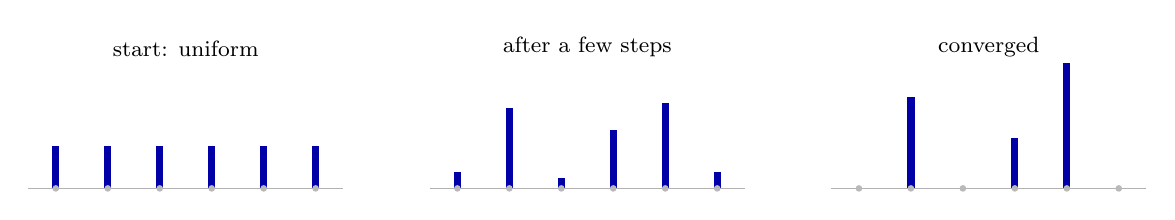
\begin{tikzpicture}[scale=1.0]
\foreach \dx/\lab/\ws in {%
  0/{start: uniform}/{0.16,0.16,0.16,0.16,0.16,0.16},
  5.1/{after a few steps}/{0.06,0.30,0.04,0.22,0.32,0.06},
  10.2/{converged}/{0.00,0.34,0.00,0.19,0.47,0.00}} {
  \begin{scope}[xshift=\dx cm]
    \node[anchor=south] at (2.0,1.55) {\footnotesize \lab};
    \draw[gray!60] (0,0) -- (4.0,0);
    \foreach \w [count=\i from 0] in \ws {
      \pgfmathsetmacro\h{\w*3.4}
      \ifdim\h pt>0.01pt
        \draw[blue!65!black,line width=2.6pt] ({0.35+\i*0.66},0) -- ({0.35+\i*0.66},\h);
      \fi
      \fill[gray!55] ({0.35+\i*0.66},0) circle (1.2pt);
    }
  \end{scope}
}
\end{tikzpicture}
\caption{How the optimal design is found. Every candidate starts with equal weight, and each
step multiplies a candidate's weight by how informative it is relative to the current average,
then renormalizes. Weights therefore stay positive and keep summing to one by construction, and
the criterion increases at every step. Candidates that are not worth running decay to zero, so
the answer is a handful of settings out of hundreds. The final weights are the fraction of
bubbles to run at each setting, and \cref{fig:certificate-schematic} is what certifies that no
other allocation does better.}
\label{fig:multiplicative}
\end{figure}

\subsection*{Designing over measures, and certifying the answer}
\label{sec:measure}

Every design result above shares a defect that no amount of care in computing them repairs:
each is the output of a search over a single design point, that search is not convex, and
nothing in its output distinguishes a good answer from a bad one. The evidence that this is
not hypothetical is in the preceding subsections. A surrogate search recovered $16\%$ of the
best conditioning actually available and reported the result without qualification; a dense
grid over a criterion whose inner minimization was unreliable produced a front that was
precise and wrong. Both look exactly like success.

The classical formulation removes the defect rather than mitigating it.

\paragraph{Designs as measures.}
Instead of choosing one design $x$ from a candidate set $\mathcal{X}$, choose a probability
measure $\xi$ on $\mathcal{X}$: run a fraction $\xi_i$ of the bubbles at setting $x_i$. This
is not an abstraction imposed for mathematical convenience -- it is what an experimenter
with a run budget does anyway, and it is strictly more expressive, since a single design is
the special case of a measure concentrated on one point. The information available from a
run allocated by $\xi$ is the average
%
\begin{equation}
M(\xi) \;=\; \sum_i \xi_i\, M(x_i),
\qquad
M(x) = J(x)^{\mathsf T}J(x),
\label{eq:measure-information}
\end{equation}
%
because information from independent runs adds and $\xi$ says how many of each to take.

The consequence is the whole point: $M(\xi)$ is \emph{linear} in $\xi$.

\paragraph{Concavity, and why the first-order condition is enough.}
$\log\det$ is concave on the positive-definite cone, and the composition of a concave
function with a linear map is concave, so $\Phi(\xi) = \log\det M(\xi)$ is concave on the
simplex -- a convex set. A concave function on a convex set has no local maximum that is
not global, and its first-order condition is not merely necessary but sufficient. Every
pathology this study ran into -- wrong basins, surrogate blind spots, answers that improve
whenever the optimizer does -- is a symptom of non-convexity, and none of them can occur
here.

The same holds for $\Phi_A = -\operatorname{tr}M(\xi)^{-1}$ and $\Phi_E =
\lambda_{\min}(M(\xi))$, and for any non-negative combination of concave criteria.

\paragraph{The directional derivative.}
Move mass $\alpha$ from $\xi$ toward the single design $x$, giving
$\xi_\alpha = (1-\alpha)\xi + \alpha\,\delta_x$. By linearity
$M(\xi_\alpha) = (1-\alpha)M(\xi) + \alpha M(x)$, and using
$\partial \log\det A = \operatorname{tr}(A^{-1}\partial A)$,
%
\begin{equation}
\phi(x,\xi) \;\equiv\; \left.\frac{\partial}{\partial\alpha}\log\det M(\xi_\alpha)\right|_{\alpha=0}
= \operatorname{tr}\!\left[M(\xi)^{-1}M(x)\right] - p .
\label{eq:directional}
\end{equation}
%
For a linear utility $u$ averaging over the design, the same construction gives
$\phi_u(x,\xi) = u_x - u^{\mathsf T}\xi$.

\paragraph{The General Equivalence Theorem.}
Since $\Phi$ is concave and the simplex is the convex hull of its vertices $\delta_x$, the
measure $\xi^\star$ maximizes $\Phi$ if and only if no vertex direction ascends:
%
\begin{equation}
\boxed{\;
\xi^\star \text{ is D-optimal}
\iff
d(x,\xi^\star) \equiv \operatorname{tr}\!\left[M(\xi^\star)^{-1}M(x)\right] \le p
\quad\text{for all } x\in\mathcal{X},
\;}
\label{eq:equivalence}
\end{equation}
%
with equality at every support point of $\xi^\star$. This is the theorem of Kiefer and
Wolfowitz~\citep{kiefer1960equivalence}, and it is what this section exists to obtain: a
quantity computed from a candidate answer that \emph{proves} the answer optimal. The gap
$\max_x d(x,\xi) - p$ is a certificate, not a convergence report.

Two further facts come free. Equality puts the support exactly where $d(x,\xi^\star)$ is
largest, so the optimal design runs at the settings of greatest standardized prediction
variance. D-optimality and G-optimality coincide.
And by Carath\'eodory's theorem applied to the convex hull of the $M(x)$, an optimal measure
supported on at most $p(p+1)/2 + 1$ points always exists: at most $11$ here.

\paragraph{Computing it.}
The implementation uses the multiplicative algorithm of Silvey, Titterington and
Torsney~\citep{silvey1978algorithm},
%
\begin{equation}
\xi_i \;\longleftarrow\; \frac{\xi_i\,F_i}{\sum_j \xi_j F_j},
\qquad
F_i = \operatorname{tr}\!\left[M(\xi)^{-1}M(x_i)\right]
\;\;\text{for}\;\; \Phi = \log\det,
\label{eq:multiplicative}
\end{equation}
%
which stays on the simplex by construction: weights remain non-negative and normalized
without projection, and the criterion rises at each step. Note that
$\sum_i \xi_i F_i = p$ identically, so~\eqref{eq:multiplicative} moves mass toward designs
whose $d(x,\xi)$ exceeds $p$, which is precisely the set that~\eqref{eq:equivalence} says
must be empty at the optimum. The update and the certificate are the same quantity.

Vertex-direction steps with a line search were tried first and cannot converge here. The step
required near the optimum falls below any fixed search grid, and the iteration stalls with a
positive gap.

Convergence of~\eqref{eq:multiplicative} degrades as candidates crowd together. A design just
off the support is nearly as good as one on it, and its weight decays in proportion.
Certifying a parabola on $[-1,1]$ took $6400$ iterations over $51$ candidates, $25\,000$ over
$101$, and $329\,000$ over $401$ -- with the criterion value correct to six figures long
before any of those.

An exhausted budget therefore yields a converged value without a proof. That is a different
thing from a wrong answer, and the reported gap distinguishes them.

\paragraph{The certified design for these records.}
Over $480$ candidates spanning $R_{\max} \in [50, 1200]\,\mu$m and stretch $[3, 20]$, with
$M(x) = J^{\mathsf T}J$ for the four qSLS parameters at the posterior median, the algorithm
certifies at a gap of $9\times10^{-10}$ in $1406$ iterations:
$\max_x \operatorname{tr}[M^{-1}M(x)] = 4.00000000$ against $p = 4$. The optimal measure is

\begin{center}
\begin{tabular}{lcc}
\toprule
$R_{\max}$ & stretch & weight \\
\midrule
$1015\,\mu$m & $6.70$ & $0.470$ \\
$161\,\mu$m  & $19.26$ & $0.303$ \\
$50\,\mu$m   & $17.78$ & $0.227$ \\
\bottomrule
\end{tabular}
\end{center}

against a best single design of $1015\,\mu$m at stretch $6.70$. The measure exceeds it by
$6.99$ in $\log\det$, a D-efficiency ratio of $\exp(6.99/4) = 5.74$; equivalently the
confidence ellipsoid is $\exp(6.99/2) \approx 33$ times smaller in volume, and a typical
parameter's interval is $\exp(6.99/8) = 2.4$ times tighter. No single design can match it,
and this is not a claim about the search: \eqref{eq:equivalence} certifies that none exists.

\begin{figure}[htbp]
\centering
\includegraphics[width=\textwidth]{fig_certificate.pdf}
\caption{The equivalence-theorem certificate. Left: the sensitivity
$d(x,\xi^\star)=\operatorname{tr}[M(\xi^\star)^{-1}M(x)]$ over the design plane, with the
three support points circled and labeled by weight; the dashed contour is the level $p=4$.
Right: the same values sorted. No design exceeds the bound and the support attains it
exactly, which is the proof -- $\max_x d = 4.00000000$ against $p=4$, gap
$9\times10^{-10}$. Nothing analogous exists for the single-design searches elsewhere in
this document.}
\label{fig:certificate}
\end{figure}

\paragraph{The mixture is the resolution of the conflict.}
The support is worth reading physically. Nearly half the runs go to a large, gently driven
bubble and the rest to small, hard-driven ones -- the two corners the earlier subsections
found pulling in opposite directions. Separating $g$ from $\alpha$ wants a gentle collapse,
because the distinguishing term of $Z_e$ decays as $\lambda^{-4}$; exciting the relaxation
mode wants a fast one.

A single design must choose between them. A measure need not. So the trade-off that motivated
the Pareto front dissolves once the design space is the one the experiment actually admits --
the front was answering a question made hard by an artificial restriction.

\paragraph{Discrimination in the same frame.}
Log evidence is additive over independent experiments, so an expected log Bayes factor per
run is linear in $\xi$ and therefore concave. The compound criterion
%
\begin{equation}
\Phi_\beta(\xi) = (1-\beta)\log\det M(\xi) + \beta\, u^{\mathsf T}\xi,
\qquad \beta \in [0,1],
\label{eq:compound}
\end{equation}
%
is then concave for every $\beta$ and inherits the certificate unchanged. Its directional
derivative is the matching combination of~\eqref{eq:directional} and $u_x - u^{\mathsf T}\xi$.
This is the compound-criterion construction of Atkinson and of Cook and
Wong~\citep{atkinson2008dt,cook1994equivalence} -- the principled form of the trade this study
otherwise handled by search.

Sweeping $\beta$ traces the Pareto front, and each criterion being concave in $\xi$ makes that
front convex. This is why the classical literature scalarizes with weighted sums where this
study needed a Chebyshev form. The non-convexity that forced the elaborate scalarization was
an artifact of optimizing over a single design point.

\paragraph{What this does not fix.}
Three limitations, stated plainly. The information matrices are evaluated at a point estimate
of $\theta$, so the design is locally optimal in the parameters though globally optimal in
$\xi$. A prior average over $\theta$ restores the guarantee at proportionate cost, since the
average of concave criteria is concave.

The candidate set is still a grid, so the certificate proves optimality \emph{over that grid}.
But $d(x,\xi^\star)$ can be evaluated anywhere, which makes checking for a missed region a
cheap scan rather than another search.

The compound form was not run on these records. The per-design log Bayes factor still suffers
the boundary pinning described above.


\begin{figure}[t]
\centering
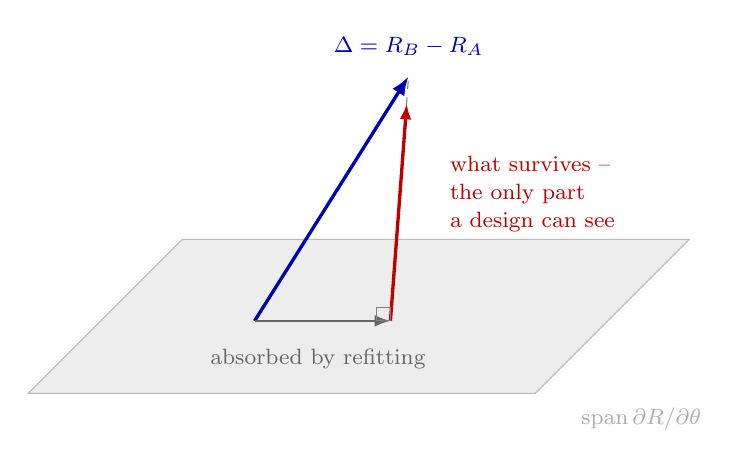
\begin{tikzpicture}[scale=1.15]
  \fill[gray!14] (0,0) -- (5.6,0) -- (7.3,1.7) -- (1.7,1.7) -- cycle;
  \draw[gray!55] (0,0) -- (5.6,0) -- (7.3,1.7) -- (1.7,1.7) -- cycle;
  \draw[-{Latex[length=2.4mm]},very thick,blue!70!black] (2.5,0.8) -- (4.2,3.5);
  \draw[-{Latex[length=2mm]},thick,gray!80!black] (2.5,0.8) -- (4.0,0.8);
  \draw[dashed,gray] (4.0,0.8) -- (4.2,3.5);
  \draw[-{Latex[length=2mm]},very thick,red!75!black] (4.0,0.8) -- (4.18,3.2);
  \draw[gray] (3.85,0.8) rectangle (4.0,0.95);
  % labels, each with its own clear lane
  \node[blue!70!black,anchor=south] at (4.2,3.62) {\footnotesize $\Delta = R_B - R_A$};
  \node[gray!65,anchor=north west] at (6.0,-0.05) {\footnotesize $\operatorname{span}\partial R/\partial\theta$};
  \node[gray!80!black,anchor=north] at (3.2,0.6) {\footnotesize absorbed by refitting};
  \node[red!75!black,anchor=west,align=left] at (4.55,2.2)
    {\footnotesize what survives --\\[-2pt]\footnotesize the only part\\[-2pt]\footnotesize a design can see};
\end{tikzpicture}
\caption{Why a model difference can be invisible at every design. Changing a model perturbs
the trace by $\Delta = R_B - R_A$. The component lying in the span of the material
sensitivities is reproduced by adjusting $g,\mu,\lambda_1,\alpha$ -- refitting absorbs it, and
no experiment recovers it. Only the orthogonal remainder is evidence that the model changed.
Measured on the \SI{15}{\celsius} record and reported in \cref{sec:axes}: the bubble-dynamics
operator is $77.7\%$ absorbed, leaving under two noise units, which is why its ranking proved
so fragile; the constitutive and thermal axes leave $8.1$ and $8.5$.}
\label{fig:absorption}
\end{figure}

\section{What the design survives}
\label{sec:survives}

The certified measure of \cref{sec:design} is a theorem. Three things stand between it and an
experiment somebody can run, and each is measurable rather than arguable.

\subsection*{A measure assigns weights; an experiment runs integers}

The optimum splits runs three ways. With twelve bubbles that is $5.4/3.7/2.9$, and the
equivalence theorem certifies optimality over \emph{measures} --- an exact design is not one,
so the certificate does not reach it. \texttt{pyimr.measure.apportion} closes the gap by the
efficient rounding of Pukelsheim and Rieder, and because that rule carries no guarantee at
small budgets, it reports the D-efficiency it achieved rather than asserting one.

On the four-point design of cubic regression, where every quantity is closed form: budgets
divisible by four lose nothing, and six runs give $2/2/1/1$ at an efficiency of $0.9428$, which
is $\left[(2/6)^2(1/6)^2/(1/4)^4\right]^{1/4}$ exactly. The rule earns its complexity on
awkward budgets --- at weights $0.7/0.2/0.1$ and four runs, proportional rounding gives
$3/1/0$, dropping a support point and leaving the information matrix singular.

\subsection*{Frames are a design variable, and there are far too many of them}

\Cref{sec:limitations} reports $201$ samples carrying the information of about ten. Redundancy
is a design variable: a camera trades frame rate against window length, against exposure, and
against how many bubbles fit in a session. Scoring frames by $\log\det J^{\mathsf T}J$ at the
fitted qSLS, with the same number of observations spent each way:

\begin{center}
\begin{tabular}{lccc}
\toprule
observations & uniform & optimally placed & gain \\
\midrule
$201$ & $18.54$ & $25.72$ & $6.0\times$ \\
$50$ & $11.73$ & $20.15$ & $8.2\times$ \\
$12$ & $5.98$ & $14.42$ & $8.3\times$ \\
\bottomrule
\end{tabular}
\end{center}

\noindent The D-optimal measure over the $201$ candidate times is certified at a gap of
$10^{-10}$ on \emph{six} support points. Fifty observations placed on those six carry more
information than all $201$ spread uniformly.

That is a measurement of slack, not a recommendation. A design on six distinct times leaves no
degrees of freedom to notice the model is wrong, and the lack-of-fit test above is exactly what
those degrees of freedom buy. The honest reading is that frames are cheap relative to their
information, so the camera should be traded for something scarce --- bubbles, or window, or
the replication that makes \eqref{eq:lackoffit} possible.

\subsection*{The recommended geometries do not survive model error}

Optimal designs are computed assuming the model is right. Ours is not: \eqref{eq:lackoffit}
says so at every temperature. The literature on sloppy systems warns that a model can fit worse
on data from its own optimal experiment, and that is testable before a bubble is spent.

The test must not generate data from the model being fitted --- that is the assumption under
examination, and a study that makes it finds nothing. So the truth carries physics the fitted
model lacks, and cold one-mode qSLS is fitted to it at four geometries. Two mismatches are
used, because one would not distinguish a property of the design from a property of the
missing physics: thermal transport, which \cref{sec:axes} sizes at $16$ noise units, and a
second relaxation mode, at $14.4$.

\begin{center}
\begin{tabular}{lcccccc}
\toprule
& \multicolumn{3}{c}{thermal truth} & \multicolumn{3}{c}{two-mode truth} \\
\cmidrule(lr){2-4}\cmidrule(lr){5-7}
geometry & $\chi^2/N$ & $g\alpha$ err & model err & $\chi^2/N$ & $g\alpha$ err & model err \\
\midrule
performed, \SI{277}{\micro\metre} at $7.09$ & $1.231$ & $\mathbf{3.8\%}$ & $0.53$ & $0.905$ & $5.0\%$ & $\mathbf{0.11}$ \\
E-optimal, \SI{199}{\micro\metre} at $3.55$ & $2.533$ & $5.9\%$ & $1.24$ & $0.877$ & $4.9\%$ & $0.19$ \\
discrimination-optimal, \SI{100}{\micro\metre} at $20.0$ & $2.197$ & $\mathbf{37.1\%}$ & $1.17$ & $1.915$ & $\mathbf{60.7\%}$ & $1.06$ \\
measure support, \SI{60}{\micro\metre} at $18.0$ & $0.892$ & $5.2\%$ & $0.15$ & $0.909$ & $\mathbf{43.5\%}$ & $0.25$ \\
\bottomrule
\end{tabular}
\end{center}

\noindent One result holds under both mismatches, and it is the strongest thing here. The
\textbf{discrimination-optimal geometry is worse on both counts, both times}: it fits $1.8$ and
$2.1$ times worse than the geometry already performed, and recovers $g\alpha$ $9.8$ and $12.2$
times worse. A design chosen to separate constitutive models degrades the parameter it was
supposed to help measure, whichever physics is missing.

The rest does not survive the change of mismatch, and saying so is the point of running two.
Under thermal error the E-optimal geometry loses on both counts; under constitutive error it is
indistinguishable from the performed one ($0.97$ and $0.98$). The \SI{60}{\micro\metre} support
point reverses more sharply: it carries the least model error under thermal truth and recovers
$g\alpha$ $8.7$ times worse under two-mode truth.

So the sloppy-systems warning is not simply confirmed. What these records support is narrower
and, for a collaborator, worse: \emph{which design is safe depends on which physics is missing,
and we do not know which is missing}. \Cref{eq:lackoffit} says the model is inadequate on every
record; it does not say in what direction. A design cannot be certified robust without naming
the model error it is robust to, and no criterion in \cref{sec:design} takes model error as an
argument at all.

The mechanism is visible in the model-error columns. A criterion computed under the
correct-model assumption sends the experiment where the model is most \emph{sensitive}, which is
often where it is most \emph{wrong}: the thermal mismatch grows from $0.53$ noise units at the
performed geometry to $1.24$ at the E-optimal one, and the fitted parameters absorb it. That
mechanism is general. Which geometry it punishes is not.

\section{Temperature dependence}

The most informative result is not any single number but a trend
(\Cref{fig:trend}). The advantage that the stiffening term buys over pure relaxation
shrinks monotonically as the gel warms: the gap between \texttt{SLS} and \texttt{qSLS}
falls from $2.94$ versus $1.35$ at \SI{15}{\celsius} to $1.41$ versus $1.23$ at
\SI{33}{\celsius}. A warmer, softer gel needs less strain-stiffening to explain its
record. Because this is a trend across three independent datasets rather than a single
fitted value, it is harder to attribute to a fitting artifact than any individual
$\chi^2$.

\begin{figure}[htbp]
\centering
\includegraphics[width=0.5\textwidth]{fig_trend.pdf}
\caption{What the stiffening term buys, against temperature. The advantage of
\texttt{qSLS} over \texttt{SLS} narrows as the gel warms.}
\label{fig:trend}
\end{figure}

\section{Conclusions}

We have treated the model comparison in inertial microcavitation rheometry as the object of
study rather than a step toward a parameter value. Ranking by evidence in coordinates the
records can answer, three findings hold.

The shear modulus is not identified separately from the stiffening exponent, so a reported
modulus is a statement about the prior box. The bubble-dynamics operator assumed throughout
this literature is beaten on every record. And a correlated residual that has been read as
constitutive model error survives every constitutive, observational and operator change tested
here.

Two of those findings needed qualifying once the equilibrium radius was fitted rather than
asserted. Compressibility is required on every record at every prior width, by $74$ to $179$
nats. Gilmore still beats the pressure form at \SI{15}{\celsius}. But at \SI{23}{\celsius} and
\SI{33}{\celsius} the operator margins collapse to under a nat, so those records never
discriminated operators at all -- pinning $R_{\mathrm{eq}}$ is what made it appear they did.
The fit wants $R_{\mathrm{eq}}$ \SIrange{3}{11}{\percent} larger than inferred, consistently
across six operators and three records, and we cannot yet explain the trend with temperature.

\subsection{Limitations of this work}
\label{sec:limitations}

\paragraph{The dropped points are outside the model, not outside the solver.}
Roughly one point in six of the winner's parameter box cannot be integrated, and that is not
a numerical shortcoming. In that region the model expands to $R/R_0 = 2132$ after its collapse
-- identically at relative tolerances of $10^{-3}$, $10^{-4}$ and $10^{-5}$. So it is a
converged property of the equations, not an artifact. The bubble begins at its maximum radius
and its energy is finite, so growth of that size is the constitutive model failing. Refusing
those points is the correct outcome.

The count of admissible points is pinned near $1958$ of $2401$ sampled whatever the settings.
Looser tolerances and a $20\times$ step budget convert failures into runaways, never into
usable solves. This corrects an earlier reading of the same failures as a stiffness problem.
The dropped points cannot be recovered by numerical effort, and no claim about the winner's
fit should be made in that region.

\begin{figure}[htbp]
\centering
\includegraphics[width=0.58\textwidth]{fig_failure_map.pdf}
\caption{Where the winner can be integrated, at the fitted modulus and viscosity. Failure is
governed principally by the stiffening, and the threshold falls to its lowest where the
relaxation time is comparable to the bubble's own period -- but it is a boundary that moves,
not an isolated band.}
\label{fig:failure}
\end{figure}

\paragraph{The ranking survives; the parameter estimates do not.}
Independent sequential Monte Carlo runs give the winner $2173.55 \pm 0.19$ in log evidence
against $2071.90 \pm 0.38$ for the relaxation-only model -- a gap of $101.6$ against
run-to-run noise near $0.4$, so the comparison is resolved by a wide margin. The tensor grid
cannot say this on its own: it returns a single number with no uncertainty.

The same grid cannot estimate parameters. Refining it from $12$ to $20$ points per axis moves
the log evidence by $17.3$, and moves the best-fit point from $g = 658$, $\alpha = 1.52$ to
$g = 144$, $\alpha = 8.86$. The best cell is simply whichever node lands nearest the ridge.

Refinement cannot fix this. The posterior standard deviations are $0.0018$, $0.0025$, $0.0055$
and $0.078$ in unit coordinates, against a grid spacing of $0.053$. The posterior therefore
occupies about $10^{-7}$ of the prior volume, and a uniform grid would need of order $10^{10}$
points. Discretization error of $17.3$ sits well inside the $101.6$ gap, so the ranking is
safe; the reported best-fit parameters are not.
\Cref{fig:coverage} shows which models lose points.

\begin{figure}[htbp]
\centering
\includegraphics[width=0.5\textwidth]{fig_coverage.pdf}
\caption{Fraction of each model's parameter grid that could not be integrated. Models not
shown lost no points.}
\label{fig:coverage}
\end{figure}

\paragraph{Consequences for the numbers reported here.}
Three methods that resolve the posterior -- sampling, a refined grid, and continuous
optimization -- agree that $g$ lies near $10^2$\,Pa. The coarse grid used for the ranking
reports $2154$\,Pa. The ranking does not depend on this; any material property quoted from the
grid does.

A modulus that size is also implausibly soft for gelatin. That is the degeneracy above making
itself felt: the fit buys a lower residual by trading modulus against stiffening, along a
direction the data barely constrain.

\paragraph{One candidate was never genuinely exercised.}
The Gent solid appears in the comparison but cannot be tested on these records. Its energy
diverges as $I_1 - 3 \to J_m$, and a Gent solid soft enough to be distinguishable from
Neo-Hookean predicts a collapse it cannot sustain, so it locks up. Where it does
integrate, it differs from Neo-Hookean by $1.7\times10^{-4}$ of $R_{\max}$ against
measurement noise near $2\times10^{-2}$ -- two orders of magnitude below what the data can
resolve. Any statement about strain-stiffening laws here excludes it.

\appendix

\section{Statistical background}
\label{app:background}

This appendix develops, from first principles, the results the main text uses. It is
self-contained and assumes only calculus and elementary probability.

\subsection{Inference as conditioning}

Write $\theta$ for parameters, $y$ for data, $M$ for a model. The product rule
$p(\theta, y) = p(y\mid\theta)\,p(\theta) = p(\theta\mid y)\,p(y)$ rearranges to Bayes'
theorem,
%
\begin{equation}
p(\theta \mid y, M) = \frac{p(y\mid\theta,M)\,\pi(\theta\mid M)}{p(y\mid M)},
\qquad
p(y\mid M) = \int p(y\mid\theta,M)\,\pi(\theta\mid M)\,\mathrm{d}\theta .
\label{eq:bayes}
\end{equation}
%
The denominator is a normalizing constant in $\theta$, which is why it is ignored when
estimating parameters and why it is the entire content of model comparison: applying
\eqref{eq:bayes} at the level of models gives
%
\begin{equation}
\frac{p(M_1\mid y)}{p(M_2\mid y)}
= \underbrace{\frac{p(y\mid M_1)}{p(y\mid M_2)}}_{\text{Bayes factor } B_{12}}
  \cdot \frac{p(M_1)}{p(M_2)} .
\end{equation}
%
Everything the data say about which model to prefer is in $B_{12}$. Jeffreys' conventional
reading takes $\log B > 1$ as substantial and $\log B > 5$ as decisive; the gap reported
here is over $100$, which is why its numerical resolution had to be checked rather than
assumed.

\subsection{The score, and two definitions of information}

Let $\ell(\theta) = \log p(y\mid\theta)$. The \emph{score} is $u = \nabla_\theta \ell$. Since
$\int p(y\mid\theta)\,\mathrm{d}y = 1$ for every $\theta$, differentiating under the integral
gives
%
\begin{equation}
\mathbb{E}_\theta[u] = \int \frac{\nabla p}{p}\,p \,\mathrm{d}y
= \nabla\!\int p \,\mathrm{d}y = 0 ,
\end{equation}
%
so the score has zero mean at the true parameter. Its covariance defines the Fisher
information, $F = \mathbb{E}[uu^{\mathsf T}]$. Differentiating the same identity twice gives
the equivalent and more useful form
%
\begin{equation}
F = \mathbb{E}\!\left[-\nabla^2\ell\right],
\end{equation}
%
the expected curvature. The two agree because
$\nabla^2\log p = \nabla^2 p/p - (\nabla p/p)(\nabla p/p)^{\mathsf T}$ and the first term
integrates to zero. Curvature and variance-of-score are the same object, which is the
reason a sharply peaked likelihood and a precisely determined parameter are the same
statement.

\subsection{The Cram\'er--Rao bound}

For an unbiased estimator $\hat\theta(y)$, differentiate
$\mathbb{E}[\hat\theta] = \theta$ under the integral to get
$\mathbb{E}[\hat\theta\,u^{\mathsf T}] = I$. Applying the Cauchy--Schwarz inequality to the
pair $(\hat\theta - \theta,\; u)$ in the scalar case gives
$\operatorname{Var}(\hat\theta)\,\mathbb{E}[u^2] \ge 1$, i.e.
$\operatorname{Var}(\hat\theta)\ge 1/F$; the multivariate statement is
%
\begin{equation}
\operatorname{Cov}(\hat\theta) \succeq F^{-1} .
\end{equation}
%
So $F^{-1}$ is a floor on achievable precision, attained asymptotically by maximum
likelihood: $\sqrt{N}(\hat\theta_N - \theta) \to \mathcal{N}(0, F_1^{-1})$ under regularity.
This is the license for reading $F^{-1}$ as a covariance and its eigenvectors as the axes of
a confidence ellipsoid -- and the regularity conditions are exactly what near-singular $F$
threatens, which is why sloppiness is worth detecting rather than tolerating.

\subsection{Gaussian data, and why $F = J^{\mathsf T}J$}

With independent Gaussian observations of known deviation,
$\ell = -\tfrac12\sum_i (y_i - m_i(\theta))^2/\sigma_i^2 + \text{const}$. Then
%
\begin{equation}
\frac{\partial \ell}{\partial\theta_j}
= \sum_i \frac{y_i - m_i}{\sigma_i^2}\frac{\partial m_i}{\partial\theta_j},
\qquad
-\frac{\partial^2\ell}{\partial\theta_j\partial\theta_k}
= \sum_i \frac{1}{\sigma_i^2}
  \left[\frac{\partial m_i}{\partial\theta_j}\frac{\partial m_i}{\partial\theta_k}
  - (y_i - m_i)\frac{\partial^2 m_i}{\partial\theta_j\partial\theta_k}\right].
\end{equation}
%
Taking the expectation kills the second bracket because $\mathbb{E}[y_i - m_i] = 0$, leaving
$F = J^{\mathsf T}J$ with $J_{ij} = \sigma_i^{-1}\partial m_i/\partial\theta_j$. Note what
was discarded: the curvature of the model. At the optimum the residuals are small and the
Gauss--Newton form is accurate; far from it, or with a badly misspecified model, $F$ and the
observed Hessian differ, and the discrepancy is itself a diagnostic.

\subsection{The Laplace approximation and the Occam factor}

To evaluate $Z = \int e^{\ell(\theta)}\pi(\theta)\,\mathrm{d}\theta$, expand about the
maximum $\hat\theta$ where $\nabla\ell = 0$:
%
\begin{equation}
\ell(\hat\theta + \delta) = \ell(\hat\theta)
  - \tfrac12\delta^{\mathsf T}H\delta + O(\|\delta\|^3),
\qquad H = -\nabla^2\ell(\hat\theta).
\end{equation}
%
Holding $\pi$ constant over the peak and using
$\int e^{-\delta^{\mathsf T}H\delta/2}\mathrm{d}\delta = (2\pi)^{p/2}|H|^{-1/2}$,
%
\begin{equation}
Z \simeq e^{\ell(\hat\theta)}\,\pi(\hat\theta)\,(2\pi)^{p/2}\,|H|^{-1/2} .
\label{eq:laplace-app}
\end{equation}
%
The correction is $O(N^{-1})$ relative for regular problems. Writing the posterior volume as
$V_{\rm post} = (2\pi)^{p/2}|H|^{-1/2}$ and the prior density as $1/V_{\rm prior}$ where it
is flat, the second factor is $V_{\rm post}/V_{\rm prior}$: the fraction of the space the
data leave standing. A model with more parameters has a larger $V_{\rm prior}$ and pays for
it unless the fit improves enough to compensate. Nothing was added by hand; the penalty is
the Jacobian of the integral.

Taking logarithms of~\eqref{eq:laplace-app}, using $H \approx N F_1$ for $N$ independent
observations, and dropping terms that do not grow with $N$,
%
\begin{equation}
-2\log Z \simeq -2\ell(\hat\theta) + p\log N + O(1),
\end{equation}
%
which is the Bayesian information criterion. BIC is therefore not an alternative to the
evidence but a coarse asymptotic of it, valid when the posterior is Gaussian, the parameters
identified, and $N$ large. AIC answers a different question -- expected out-of-sample
Kullback--Leibler divergence -- and is not an approximation to $Z$ at all. Where a model is
sloppy, $H$ is near-singular, $|H|^{-1/2}$ is enormous, and the asymptotic form fails while
the integral remains well defined.


\begin{figure}[t]
\centering
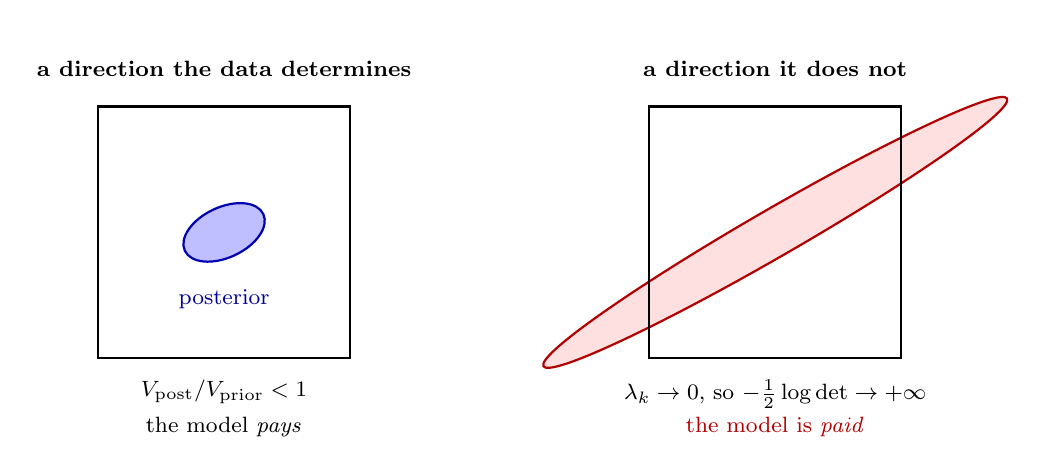
\begin{tikzpicture}[scale=1.0]
\begin{scope}
  \node[anchor=south] at (1.6,3.45) {\footnotesize\textbf{a direction the data determines}};
  \draw[thick] (0,0) rectangle (3.2,3.2);
  \fill[blue!25,draw=blue!70!black,thick,rotate around={25:(1.6,1.6)}] (1.6,1.6) ellipse (0.55 and 0.32);
  \node[blue!60!black] at (1.6,0.75) {\footnotesize posterior};
  \node[anchor=north] at (1.6,-0.15) {\footnotesize $V_{\rm post}/V_{\rm prior}<1$};
  \node[anchor=north] at (1.6,-0.62) {\footnotesize the model \emph{pays}};
\end{scope}
\begin{scope}[xshift=7.0cm]
  \node[anchor=south] at (1.6,3.45) {\footnotesize\textbf{a direction it does not}};
  \draw[thick] (0,0) rectangle (3.2,3.2);
  \begin{scope}
    \clip (-1.5,-1.0) rectangle (4.7,4.2);
    \fill[red!12,draw=red!70!black,thick,rotate around={30:(1.6,1.6)}] (1.6,1.6) ellipse (3.4 and 0.30);
  \end{scope}
  \draw[thick] (0,0) rectangle (3.2,3.2);
  \node[anchor=north] at (1.6,-0.15) {\footnotesize $\lambda_k\to0$, so $-\tfrac12\log\det\to+\infty$};
  \node[red!70!black,anchor=north] at (1.6,-0.62) {\footnotesize the model is \emph{paid}};
\end{scope}
\end{tikzpicture}
\caption{The Occam factor is the share of the prior the data leaves standing,
$\prod_k\sqrt{2\pi/\lambda_k}$ over the eigenvalues of $J^{\mathsf T}J$. Left: every direction
is narrower than its prior, so a flexible model pays for volume it does not use. Right: a
direction the data does not determine has $\lambda_k\to0$, the fitted Gaussian extends far
outside the box the prior occupies, and the expansion returns a factor \emph{greater} than
one -- the evidence rises when a useless parameter is added. Capping each direction at unity,
\eqref{eq:occam-capped}, restores what the geometry already required; on the models of
\cref{sec:enrich} the uncapped form favored the two-mode law by $29.7$ nats exactly where
its second arm did nothing.}
\label{fig:occam}
\end{figure}

\subsection{Capping the Occam factor at the prior}
\label{sec:occam-cap}

The failure just noted is not merely a loss of accuracy; it has a sign, and the sign is
wrong. Work in coordinates where the prior is uniform on the unit cube, so
$V_{\rm prior} = 1$ and $H = J^{\mathsf T}J$. The Occam factor is a product over the
eigendirections of $J^{\mathsf T}J$,
%
\begin{equation}
\frac{V_{\rm post}}{V_{\rm prior}} = \prod_{i=1}^{p}\sqrt{\frac{2\pi}{\lambda_i}},
\label{eq:occam-product}
\end{equation}
%
each factor being the posterior width in that direction against a prior of width one. A
direction the data does not determine has $\lambda_i \to 0$ and contributes a factor
diverging to $+\infty$. The evidence then \emph{increases} with the addition of a parameter
that does nothing, which is the opposite of what the Occam factor exists to do.

The pathology is entirely an artifact of the Gaussian approximation. The fitted Gaussian has
width $\sqrt{2\pi/\lambda_i} \gg 1$ in that direction and so extends far outside the cube the
prior actually occupies, while the true integral, taken over the cube, simply returns the
prior mass. Imposing what the geometry already requires -- a posterior cannot be wider than
the prior it came from -- gives
%
\begin{equation}
\log\frac{V_{\rm post}}{V_{\rm prior}} \;=\; \sum_{i=1}^{p}\min\!\left(0,\;
  \tfrac12\log\frac{2\pi}{\lambda_i}\right),
\label{eq:occam-capped}
\end{equation}
%
so a direction the data cannot see costs nothing and buys nothing. Where every
$\lambda_i > 2\pi$ each minimum selects its second argument
and~\eqref{eq:occam-capped} reduces identically to the logarithm
of~\eqref{eq:occam-product}: the cap is a strict generalization, altering an answer only
where the uncapped form was not entitled to one. \cref{sec:enrich} gives the size of the
error it removes, which on the models considered there is $29.7$ nats.

This matters wherever models of differing dimension are compared and some parameters are
weakly identified -- which, for the sloppy spectra of \cref{sec:sloppy}, is the normal
case rather than the exceptional one.


\begin{figure}[t]
\centering
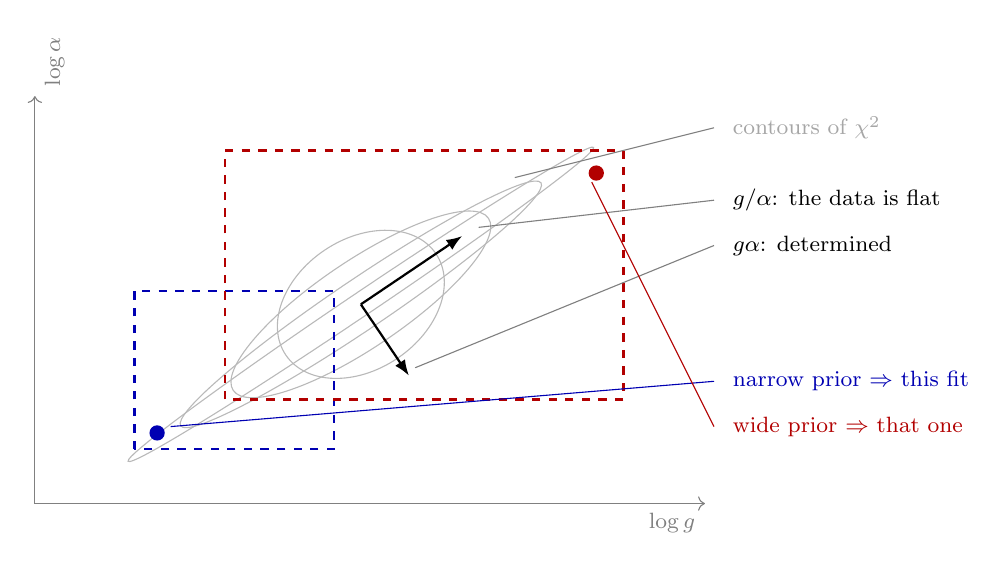
\begin{tikzpicture}[scale=1.15]
  \draw[->,gray] (0,0) -- (7.4,0) node[anchor=north east] {\footnotesize $\log g$};
  \draw[->,gray] (0,0) -- (0,4.5) node[anchor=north west,rotate=90] {\footnotesize $\log\alpha$};
  \begin{scope}
    \clip (0.05,0.05) rectangle (7.3,4.4);
    \foreach \r/\o in {3.1/0.13, 2.4/0.28, 1.7/0.48, 1.0/0.72} {
      \draw[gray!55,rotate around={34:(3.6,2.2)}] (3.6,2.2) ellipse ({\r} and {\o});
    }
  \end{scope}
  \draw[blue!70!black,thick,dashed] (1.1,0.6) rectangle (3.3,2.35);
  \draw[red!70!black,thick,dashed] (2.1,1.15) rectangle (6.5,3.9);
  \fill[blue!70!black] (1.35,0.78) circle (2.4pt);
  \fill[red!70!black] (6.2,3.65) circle (2.4pt);
  \draw[-{Latex[length=2mm]},thick] (3.6,2.2) -- ++(34:1.35);
  \draw[-{Latex[length=2mm]},thick] (3.6,2.2) -- ++(-56:0.95);
  % every label sits outside the drawing
  \node[gray!70,anchor=west] at (7.6,4.15) {\footnotesize contours of $\chi^2$};
  \node[anchor=west] at (7.6,3.35) {\footnotesize $g/\alpha$: the data is flat};
  \node[anchor=west] at (7.6,2.85) {\footnotesize $g\alpha$: determined};
  \node[blue!70!black,anchor=west] at (7.6,1.35) {\footnotesize narrow prior $\Rightarrow$ this fit};
  \node[red!70!black,anchor=west] at (7.6,0.85) {\footnotesize wide prior $\Rightarrow$ that one};
  \draw[gray] (7.5,4.15) -- (5.3,3.6);
  \draw[gray] (7.5,3.35) -- (4.9,3.05);
  \draw[gray] (7.5,2.85) -- (4.2,1.5);
  \draw[blue!70!black] (7.5,1.35) -- (1.5,0.85);
  \draw[red!70!black] (7.5,0.85) -- (6.15,3.55);
\end{tikzpicture}
\caption{Why a ``best fit'' for $g$ is a statement about the prior. The likelihood depends on
the product $g\alpha$, so the misfit surface is a valley running along constant $g\alpha$ and
the data is flat along $g/\alpha$. An optimizer slides until it meets the edge of the box, and
\emph{where} it stops is set by the box: the two dashed rectangles give the two filled points,
which differ in $g$ by more than thirtyfold. This is the mechanism behind the fifty-nat swing
in the operator ranking of \cref{sec:operator} when the bounds were widened, and behind the
order-of-magnitude disagreement in $g$ between methods in \cref{fig:valley}.}
\label{fig:ridge}
\end{figure}


\begin{figure}[t]
\centering
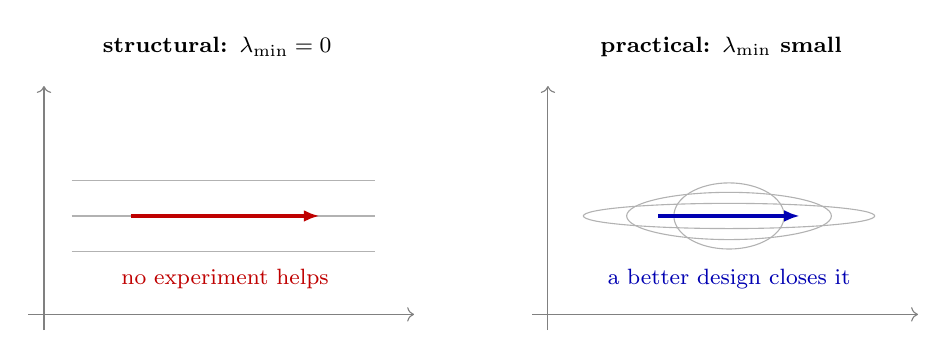
\begin{tikzpicture}[scale=1.0]
\begin{scope}
  \node[anchor=south] at (2.4,3.35) {\footnotesize\textbf{structural: $\lambda_{\min}=0$}};
  \draw[->,gray] (0,0.2) -- (4.9,0.2); \draw[->,gray] (0.2,0) -- (0.2,3.1);
  \foreach \y in {1.0,1.45,1.9} { \draw[gray!60] (0.55,\y) -- (4.4,\y); }
  \draw[-{Latex[length=2mm]},very thick,red!75!black] (1.3,1.45) -- (3.7,1.45);
  \node[red!75!black,anchor=north] at (2.5,0.9) {\footnotesize no experiment helps};
\end{scope}
\begin{scope}[xshift=6.4cm]
  \node[anchor=south] at (2.4,3.35) {\footnotesize\textbf{practical: $\lambda_{\min}$ small}};
  \draw[->,gray] (0,0.2) -- (4.9,0.2); \draw[->,gray] (0.2,0) -- (0.2,3.1);
  \foreach \r/\o in {1.85/0.16, 1.3/0.30, 0.7/0.42} {
    \draw[gray!60,rotate around={0:(2.5,1.45)}] (2.5,1.45) ellipse ({\r} and {\o});
  }
  \draw[-{Latex[length=2mm]},very thick,blue!70!black] (1.6,1.45) -- (3.4,1.45);
  \node[blue!70!black,anchor=north] at (2.5,0.9) {\footnotesize a better design closes it};
\end{scope}
\end{tikzpicture}
\caption{Two failures that look alike in a fit and differ completely in what can be done about
them. Left: the misfit is exactly flat along a direction, $F$ is singular, and the parameter
combination is structurally unidentifiable. No experiment recovers it, and only a
reparameterization or a fixed value helps. Right: the misfit is closed but very elongated, $F$
is invertible and ill-conditioned, and the combination is determined weakly. Here a design
that rotates the ellipse can close it, which is what \cref{sec:design} sets out to do. On
these records $\lambda_{\min}=5.2\times10^{-2}\neq0$, so the problem is the second kind.}
\label{fig:structural}
\end{figure}


\begin{figure}[t]
\centering
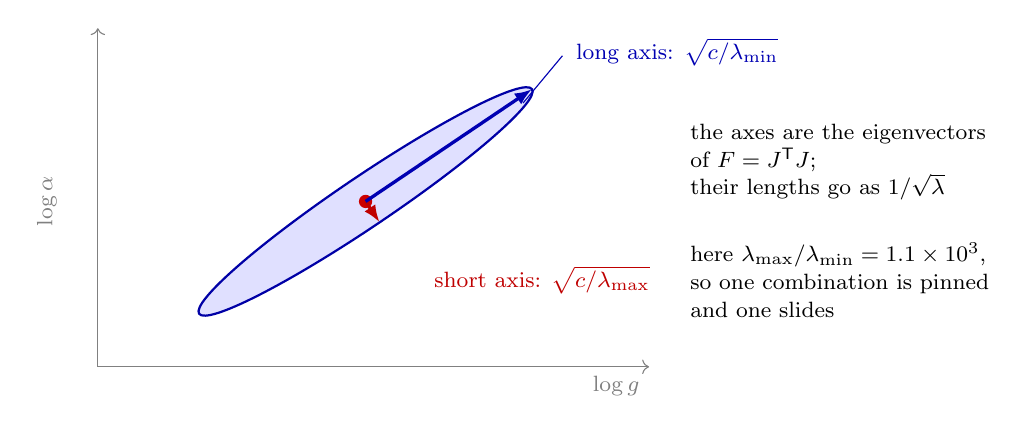
\begin{tikzpicture}[scale=1.0]
  \draw[->,gray] (0,0) -- (7.0,0) node[anchor=north east] {\footnotesize $\log g$};
  \draw[->,gray] (0,0) -- (0,4.3);
  \node[gray,rotate=90,anchor=south] at (-0.4,2.1) {\footnotesize $\log\alpha$};
  % arrows are drawn AT the semi-axis lengths, 2.55 and 0.32. An earlier version drew the
  % short one at 0.62, twice its own axis, so it stuck out of the ellipse it was measuring.
  \fill[blue!12,draw=blue!65!black,thick,rotate around={34:(3.4,2.1)}]
    (3.4,2.1) ellipse (2.55 and 0.32);
  \fill[red!80!black] (3.4,2.1) circle (2.4pt);
  \draw[-{Latex[length=2.2mm]},very thick,red!75!black] (3.4,2.1) -- ++(-56:0.32);
  \draw[-{Latex[length=2.2mm]},very thick,blue!70!black] (3.4,2.1) -- ++(34:2.55);
  \node[red!75!black,anchor=north west] at (4.15,1.4) {\footnotesize short axis: $\sqrt{c/\lambda_{\max}}$};
  \node[blue!70!black,anchor=west] at (5.95,4.0) {\footnotesize long axis: $\sqrt{c/\lambda_{\min}}$};
  \draw[blue!70!black,thin] (5.9,3.95) -- (5.4,3.35);
  \node[anchor=west,align=left] at (7.4,2.6)
    {\footnotesize the axes are the eigenvectors\\[-2pt]\footnotesize of $F=J^{\mathsf T}J$;\\[-2pt]
     \footnotesize their lengths go as $1/\sqrt{\lambda}$};
  \node[anchor=west,align=left] at (7.4,1.1)
    {\footnotesize here $\lambda_{\max}/\lambda_{\min}=1.1\times10^{3}$,\\[-2pt]
     \footnotesize so one combination is pinned\\[-2pt]\footnotesize and one slides};
\end{tikzpicture}
\caption{Why some parameter combinations are determined and others are not. Near the best fit
the misfit rises as a quadratic form, so the contour of constant misfit is an ellipse whose
axes point along the eigenvectors of $F=J^{\mathsf T}J$ and whose half-lengths go as
$1/\sqrt{\lambda}$. A large eigenvalue is a short axis: move that way and the fit degrades at
once. A small one is a long axis: move that way and the data barely object. On these records
the ratio is $1.1\times10^{3}$, and the long direction is $g$ up with $\alpha$ down at fixed
product, which is the ridge of \cref{fig:ridge} seen from above. The ellipse is drawn at an
aspect of about $8:1$; the measured aspect is $\sqrt{1.1\times10^{3}}\approx33:1$, which would
render as a line.}
\label{fig:fisher}
\end{figure}

\subsection{Sloppy models}
\label{sec:sloppy}

Write the eigen-decomposition $F = V\Lambda V^{\mathsf T}$ with
$\lambda_1 \ge \cdots \ge \lambda_p$. The misfit near the optimum is
$\Delta\chi^2 = \sum_k \lambda_k c_k^2$ for $\delta = \sum_k c_k v_k$, so moving a distance
$c$ along $v_k$ costs $\lambda_k c^2$ and the $95\%$ contour lies at
$c_k = \sqrt{3.84/\lambda_k}$. Multiparameter models of this kind generically show spectra
spanning many decades, with a few stiff directions and many sloppy ones -- the observation
of Gutenkunst~\citep{gutenkunst2007universally}, Sethna and co-workers, and the reason parameter values in such models are
often far less determined than their predictions.

The distinction to keep is between a rank-deficient $F$, where a direction is
\emph{structurally} unidentifiable and no experiment helps, and a merely ill-conditioned
$F$, where the direction is determined but weakly. In logarithmic parameters, an eigenvector
is a power-law combination, and the invariant it leaves fixed is read off its components.


\begin{figure}[t]
\centering
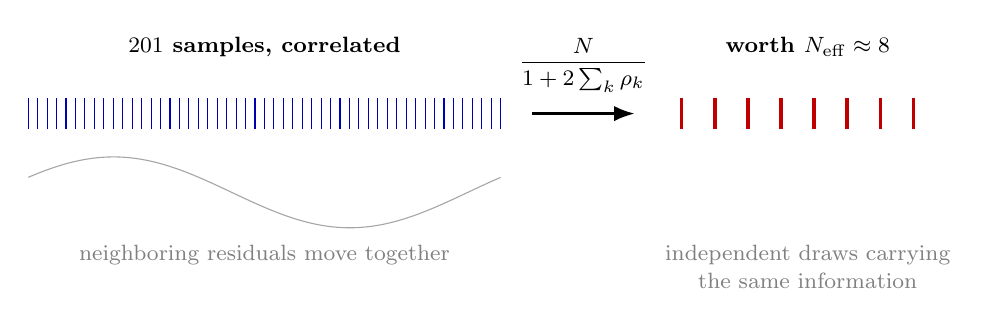
\begin{tikzpicture}[scale=1.0]
\begin{scope}
  \node[anchor=south] at (3.0,2.35) {\footnotesize\textbf{$201$ samples, correlated}};
  \foreach \i in {0,...,50} { \draw[blue!70!black] ({\i*0.12},1.55) -- ({\i*0.12},1.95); }
  \draw[gray!70,smooth,samples=60,domain=0:6] plot (\x, {0.75 + 0.45*sin(60*\x + 25)});
  \node[gray,anchor=north] at (3.0,0.2) {\footnotesize neighboring residuals move together};
\end{scope}
\begin{scope}[xshift=8.3cm]
  \node[anchor=south] at (1.6,2.35) {\footnotesize\textbf{worth $N_{\rm eff}\approx8$}};
  \foreach \i in {0,...,7} { \draw[red!75!black,very thick] ({\i*0.42},1.55) -- ({\i*0.42},1.95); }
  \node[gray,anchor=north,align=center] at (1.6,0.2)
    {\footnotesize independent draws carrying\\[-2pt]\footnotesize the same information};
\end{scope}
  \draw[-{Latex[length=2.6mm]},thick] (6.4,1.75) -- (7.7,1.75);
  \node[anchor=south] at (7.05,1.9) {\footnotesize $\dfrac{N}{1+2\sum_k\rho_k}$};
\end{tikzpicture}
\caption{Why $201$ samples do not carry $201$ samples' worth of evidence. The residuals here
are strongly correlated from one sample to the next, so neighboring points repeat information
rather than adding it. A correlated sequence carries what
$N_{\rm eff}=N/(1+2\sum_k\rho_k)$ independent draws would, and on these fits $N_{\rm eff}$ is
near $8$. Both $\chi^2/N$ and the evidence assume the samples are independent, so each
overstates the information by roughly $N/N_{\rm eff}\approx25$. A margin of a few nats between
two models is inside that factor.}
\label{fig:neff}
\end{figure}

\subsection{Correlated errors}

Let $r$ be the residual vector with covariance $C$. The Gaussian log-likelihood is
%
\begin{equation}
-2\ell = r^{\mathsf T}C^{-1}r + \log|C| + N\log 2\pi ,
\end{equation}
%
and with the Cholesky factorization $C = LL^{\mathsf T}$ this becomes
$\|L^{-1}r\|^2 + 2\sum_k\log L_{kk} + \text{const}$: whitening turns generalized least
squares back into ordinary least squares on transformed residuals. Ignoring the off-diagonal
terms, i.e. using $\operatorname{diag}(C)$, does not merely lose efficiency -- it
misstates the amount of information. For a stationary sequence with autocorrelation
$\rho_k$,
%
\begin{equation}
\operatorname{Var}\!\left(\sum_{i=1}^N r_i\right)
= N\sigma^2\left(1 + 2\sum_{k=1}^{N-1}\Big(1 - \tfrac{k}{N}\Big)\rho_k\right)
\;\xrightarrow{\;N\to\infty\;}\; N\sigma^2\left(1 + 2\sum_{k\ge1}\rho_k\right),
\end{equation}
%
so the sequence carries the information of $N_{\rm eff} = N/(1 + 2\sum\rho_k)$ independent
draws. The bracket is the spectral density of the residual sequence at zero frequency, which
is the cleaner way to see why a long-range correlation is so costly.

Correlated residuals in a \emph{fitted} model usually indicate model discrepancy rather than
correlated measurement noise. Kennedy and O'Hagan~\citep{kennedy2001bayesian} formalize this by writing
$y = m(\theta) + \delta(\cdot) + \varepsilon$ with $\delta$ a Gaussian process, and
Brynjarsd\'ottir and O'Hagan show that omitting $\delta$ leaves parameter estimates biased
\emph{and} overconfident, while an unconstrained $\delta$ absorbs the physics. Neither
failure is visible in $\chi^2$.

\subsection{Optimal experimental design}

A design $\xi$ determines what is measured and hence $F(\xi,\theta)$. Since $F$ is a matrix
and designs must be ranked, a scalar functional is required, and the classical choices are
%
\begin{equation}
\Phi_D = \log\det F, \quad
\Phi_A = -\operatorname{tr}F^{-1}, \quad
\Phi_E = \lambda_{\min}(F), \quad
\Phi_c = -c^{\mathsf T}F^{-1}c ,
\end{equation}
%
each maximized. In Bayesian terms, $\Phi_D$ is the expected Kullback--Leibler gain from
prior to posterior under a Gaussian approximation, which is why it is the default: it
maximizes information about \emph{all} parameters jointly. That default is wrong whenever
one direction is the question, because $\log\det F = \sum_k\log\lambda_k$ is dominated by
the large eigenvalues.

Because $F$ depends on $\theta$, a local design presupposes an answer. The standard repairs
are to average over a prior, $\Phi(\xi) = \mathbb{E}_\theta[\Phi(F(\xi,\theta))]$, or to
take the worst case over a plausible set. Sequential design uses the posterior from
completed experiments as the prior for the next, which is what is done here.

When the model itself is uncertain, all of the above presuppose the wrong thing. T-optimality
(Atkinson and Fedorov) maximizes instead the lack of fit of the inferior model,
%
\begin{equation}
\Phi_T(\xi) = \min_{\theta_2}\;\big\|m_1(\hat\theta_1;\xi) - m_2(\theta_2;\xi)\big\|^2 ,
\end{equation}
%
which asks which experiment the candidates most disagree about. Its virtue here is that it
shares no assumptions with the Fisher criteria, so agreement between them is evidence rather
than restatement.

\section{Reproducing}

\begin{verbatim}
.venv/bin/python examples/measured_selection.py <dataset> [thermal Nt] [workers]
.venv/bin/python docs/writeup/collect.py 16     # records results.json
.venv/bin/python docs/writeup/figures.py        # draws every figure from it
\end{verbatim}

Every number and figure in this document comes from \texttt{results.json}; none is
transcribed by hand.

\section*{Code and data availability}

Every number and figure in this document is reproduced by scripts in the repository that
contains it: \texttt{figures.py}, \texttt{figures\_geometry.py},
\texttt{figures\_identifiability.py}, \texttt{figures\_measure.py} and
\texttt{figures\_trial.py} draw the figures, \texttt{fit\_quality.py} the fit table and
\texttt{trial\_variation.py} the trial-spread analysis, each from the tracked
\texttt{results.json}. The design measures use \texttt{pyimr.measure}, the discrimination
criteria \texttt{pyimr.discriminate}, and the trade-off front \texttt{pyimr.pareto}. The
measured records themselves are not redistributed here.

\bibliographystyle{unsrtnat}
\bibliography{selection}

\end{document}
